\documentclass[twoside,11pt,openright]{report}

\usepackage[latin1]{inputenc}
\usepackage[american]{babel}
\usepackage{a4}
\usepackage{latexsym}
\usepackage{amssymb}
\usepackage{amsmath}
\usepackage{epsfig}
\usepackage[T1]{fontenc}
\usepackage{mathptmx}
\usepackage{color}
\usepackage{epstopdf}
\usepackage{microtype}
\usepackage{hyperref}
\usepackage{listings}
\usepackage{float}
\usepackage{verbatim}
\usepackage{mathpartir}
\usepackage{multirow}
\usepackage{xcolor}
\usepackage[]{quoting}
\usepackage[useregional]{datetime2}
\DTMlangsetup[en-US]{showdayofmonth=false}
\usepackage{lipsum}

\usepackage[newfloat]{minted}
\usepackage{caption}
\usemintedstyle{tango}

\newenvironment{code}{\captionsetup{type=figure, singlelinecheck=off, justification=raggedleft}}{}
\SetupFloatingEnvironment{listing}{name=Coq Code}

\renewcommand*\sfdefault{lmss}
\renewcommand*\ttdefault{txtt}

\def\@bsphack{%
  \relax
  \ifhmode
    \@savsk\lastskip
    \@savsf\spacefactor
  \fi}
\def\@esphack{%
  \relax
  \ifhmode
    \spacefactor\@savsf
    \ifdim\@savsk>\z@
      \ignorespaces
    \fi
  \fi}

% \makeatletter
% \newcommand{\todo}[1]{%
%   \@bsphack
%   \@esphack
% }
% \makeatother
%\newcommand{\todo}[1]{{\color[rgb]{.5,0,0}\textbf{$\blacktriangleright$#1$\blacktriangleleft$}}}

\newcommand{\pbt}{Property-Based Testing}
\newcommand{\cc}{ConCert}
\newcommand{\coq}[1]{\texttt{#1}}



\hypersetup{
    colorlinks=true,
    linkcolor=black,
    filecolor=magenta,      
    urlcolor=blue,
}

\definecolor{hudfarve}{RGB}{255, 234, 200}


\begin{document}

%%%%%%%%%%%%%%%%%%%%%%%%%%%%%%%%%%%%%%%%%%%%%%%%%%%%%%%%%%%%%%%%%%%%%%%

\pagestyle{empty} 
\pagenumbering{roman} 
\vspace*{\fill}\noindent{\rule{\linewidth}{1mm}\\[4ex]
{\Huge\sf Property-Based Testing of Smart\\Contracts in Coq}\\[4ex]
{\huge\sf Mikkel Milo Tromborg Nielsen, \Large{201505317/au543733}}\\[2ex]

\noindent\rule{\linewidth}{1mm}\\[4ex]
\noindent{\Large\sf Master's Thesis, Computer Science\\[1ex] 
\today \\[1ex] Advisor: Bas Spitters\\[15ex]}\\[\fill]}

\epsfig{file=logo.eps}
\clearpage

%%%%%%%%%%%%%%%%%%%%%%%%%%%%%%%%%%%%%%%%%%%%%%%%%%%%%%%%%%%%%%%%%%%%%%%

\pagestyle{plain}
\chapter*{Abstract}
\addcontentsline{toc}{chapter}{Abstract}

%%%%
%We have developed a \pbt{} framework for ConCert, a blockchain formalisation in Coq, using QuickChick. Our approach is based on automatically generating arbitrary, valid execution traces for testing from semi-automatically derived generators. 
%This means we can define testable properties over \textit{entire} execution traces, unlike existing \pbt{} which only allow testing single steps of execution on a particular contract. In particular, this approach allows us to test both functional and temporal properties of contracts, both in isolation and with multiple, interacting contracts. We have demonstrated these capabilities of our framework in various case studies such as ERC-20 tokens, the Congress, FA2 tokens, and the UniSwap token exchange platform, where we implemented these contracts in ConCert, and tested key properties on them. We used our testing framework to successfully discover well-known vulnerabilities such as a vulnerability in transfers of ERC-20 compliant tokens, the re-entrancy vulnerability on the DAO, and a recently discovered re-entrancy vulnerability in the UniSwap protocol. We found these vulnerabilities using our testing framework by stating safety properties, either as functional of temporal properties. 
%Thus, we have shown not only the feasibility of using \pbt{} on smart contracts, but also its effectiveness. We have also demonstrated how testing and verification efforts can be combined. In part, this is due to the fact that both ConCert and our testing framework are developed in the Coq proof assistant, but also because QuickChick allows, to some extent, testing on the same specification that one intends to prove. This means testing can be used as a preliminary, cost-effective step in the process of formal verifying a (collection of interacting) contract(s) in order to potentially discover bugs. We demonstrated this in our tests of the Congress contract.



%%%%%%%%%

Smart contracts are distributed applications running on a blockchain, and are typically used for sensitive transactions, for example carrying
large amounts of money. Once deployed, they are impossible to change. Hence, correctness of the smart contract implementation is imperative. One approach is to formally verify the specification using a proof assistant, but this typically requires significant effort and specialized knowledge of formal methods. In this work we take a \textit{semi-formal} approach to increasing assurance that a smart contract implementation satisfies a specification by using Property-Based Testing to test properties on automatically generated blockchain execution traces.

We demonstrate feasibility of the approach by developing a framework for Property-Based Testing of smart contracts in Coq using QuickChick, supporting testing of functional and temporal properties. We demonstrate its effectiveness at discovering bugs/vulnerabilities on various non-trivial contracts such as an ERC-20 compliant token contract, a Congress contract, and an implementation of the Tezos FA2 Token standard.

Our testing framework may either be used as a preliminary step to support formal verification, by serving as a cost effective tool to discover bugs, or as a complementary approach whenever formal verification is not an option.

% \chapter*{Resum\'e}
% \addcontentsline{toc}{chapter}{Resum\'e}

% \todo{in Danish\dots}

\chapter*{Acknowledgments}
\addcontentsline{toc}{chapter}{Acknowledgments}
I would like to thank my advisor Bas Spitters for his excellent guidance, for providing useful reference material, and for his continued, shared enthusiasm of my work. I would also like to express my gratitude to Danil Annenkov who essentially has acted as my secondary advisor throughout the entire project, and has provided indispensable feedback on this thesis. Finally, I would like to thank Jakob Botsch Nielsen, a PhD student at Aarhus University, for sparring and answering countless of my questions related to the ConCert framework, of which he is a developer of. 
% \vspace{2ex}
% \begin{flushright}
%   \emph{Bas Spitters,}\\
%   \emph{Danil Annenkov,}\\
%   \emph{Aarhus, \today.}
% \end{flushright}

\chapter*{Readers' Guide}
\addcontentsline{toc}{chapter}{Readers' Guide}
This thesis is intended to be read chronologically since each chapter depends on the preceding chapter, with only a few exceptions that we list here. For readers not familiar with QuickChick, \autoref{ch:appendix-qc-example} is recommended reading after \autoref{ch:quickchick} and before reading \autoref{ch:design-implementation}. Chapter \ref{ch:quickchick} and \autoref{ch:appendix-qc-example} \textit{can} be skipped by readers familiar with QuickChick, although it is not recommended. The case studies in \autoref{ch:case-studies} may be read independently, and it is sufficient (but not recommended) to only read a subset of them. However we highly recommend reading \autoref{sec:erc20-case-study} before the succeeding case studies. These recommendations are also stated when relevant in the following chapters.



%%%%%%%%%%%%%%%%%%%%%%%%%%%%%%%%%%%%%%%%%%%%%%%%%%%%%%%%%%%%%%%%%%%%%%
\setcounter{tocdepth}{1}
\tableofcontents
%\cleardoublepage
\pagenumbering{arabic}
\setcounter{secnumdepth}{2}

%%%%%%%%%%%%%%%%%%%%%%%%%%%%%%%%%%%%%%%%%%%%%%%%%%%%%%%%%%%%%%%%%%%%%%%

\chapter{Introduction}
\label{ch:intro}
Blockchain-based platforms are seeing rising popularity in recent years. This can be attributed by their ability to sustain a public, distributed ledger with high degrees of reliability, integrity, and inspection. All while not requiring a trusted third-party entity. In the early days of blockchain platforms such as Bitcoin, the primary concern was to support management of cryptocurrencies, however newer blockchain platforms such as Ethereum and Tezos have shifted their focus towards execution of \textit{smart contracts} on the blockchain.
Smart contracts are distributed applications running on a blockchain, and are typically used for sensitive transactions, for example carrying large amounts of money or other highly valuable assets, but they can in principle perform any computation. Once a smart contract is deployed on the blockchain, it is impossible to modify or update its source code. The blockchain ensures that contracts are executed correctly according to the underlying execution model, in particular that no adversary can intercept the execution of a contract. However, it gives no guarantee that the code of the contract is correct. Since smart contracts are essentially just programs they are of course still susceptible to bugs, like any other software. \medskip\\
A security audit on Ethereum smart contracts performed by Trail of Bits found 246 vulnerabilities in 23 contracts\cite{groce2019actual}. The three most common types of detected vulnerabilities were related to data validation, access control, and race conditions. Of these three categories, respectively $21\%$, $42\%$, and $41\%$ were classified as having ``high severety''.
There have been examples of attacks on smart contracts that have resulted major losses, such as the ``DAO attack'' on Ethereum where, at the time, \$50 million worth of cryptocurrency was stolen due to a re-entrancy vulnerability\cite{daoattack}. In 2017 a vulnerability was discovered and exploited in the Parity Wallet's multi-signature contract on the Ethereum blockchain, resulting in a loss of \$280 million worth of cryptocurrency\cite{multisighack}. More recently, in April 2020 another re-entrancy attack was conducted against the Lendf.me platform by exploiting a vulnerability when combining the usage of ERC777 compliant tokens and a UniSwap contract\cite{uniswap-exploit}.w
The attack resulted in a loss of about $99.5\%$ of the platform's funds, corresponding to about \$25 million worth of cryptocurrency. The attackers have since returned nearly all the stolen funds after negotiation with Lendf.me and the dForce Foundation.

Hence, having a high assurance that a smart contract implementation is free of bugs is imperative. There are several approaches to solve this problem. For example, software development practices such as code reviews can be integrated into the development process. Similarly, the software can be open-sourced to allow anyone to review and comment on the code. The UniSwap vulnerability was in fact already publicly disclosed and acknowledged prior to the attack\footnote{\url{https://github.com/ConsenSys/Uniswap-audit-report-2018-12\#31-liquidity-pool-can-be-stolen-in-some-tokens-eg-erc-777-29}}, which was only possible because the source code is publically available on github\footnote{\url{https://github.com/Uniswap}}. While some bugs and mistakes can be identified by peer reviews, it is unreasonable to expect humans to detect all bugs due to the intricacy of some bugs. 

The smart contract language itself may guard against certain coding mistakes through its type system. Strong type systems can ensure or significantly reduce unexpected run-time errors, and may even verify certain properties on the data operated by the programs. However by Rice's Theorem, type systems cannot verify \textit{arbitrary} properties automatically. Hence, the expressibility of type systems for programming languages are very limited.

Formal methods deals with rigorously specifying behavior in precise, mathematical languages, and verifying that an implementation satisfies this specification. There are many instances of formal methods, and we don't intend to discuss all of them. Broadly speaking, formal methods can be divided into two categories: model-checking and proof-based approaches. Both approaches deals with verifying formal properties stated as mathematical formulas. Proof-based approaches require formal semantics of the contract language and perhaps also of the execution model of the underlying blockchain. Model-checking requires that the contract is somehow represented as an executable model, typically a state machine. Needless to say, the integrity of both approaches depend entirely on correctness of the formalisations; if the semantics or execution model does not correctly represent the actual implementation, or the state machine does not correctly represent the contract, then the absolute guarantees do not apply to the actual implementation. Further formal proofs may be conducted to ensure no such discrepancies,  but it is important to understand that ultimately there must always be an unverified, trusted representation/code base. This is a fundamental limitation of formal methods, and can be viewed as an artefact of G\"odel's Second Incompleteness Theorem which, in informal terms, states that no consistent formal system can prove its own consistency.
\medskip\\
\textbf{Model-checking.} Model checking involves building a finite-state model of the program and checking if this model satisfies a specification. A popular approach is to represent the model and the \textit{negation} of the specification as temporal formulas in e.g. Linear Temporal Logic. Equivalent B\"uchi automata can be automatically derived. If the intersection of the languages represented by the two automata is empty, then the model satisfies specification. Intuitively this holds because the set of states represented by the B\"uchi automaton for the negated specification is exactly all the states that do not satisfy the specification. If the model does not intersect with any of these states, then it satisfies the specification.

Model Checking has been employed for Ethereum's Solidity smart contract language in \cite{fsolidm18} and extended in \cite{inbook} with support for formal verification. In \cite{fsolidm18} they build a tool, \textit{FSolidM}, where contracts are developed as finite state machines \textit{first}, and then later extracted to Solidity code. The tool has plug-ins that can automatically apply security patterns such as ensuring resilience against some re-entrancy attacks, or applying access control to endpoints of the contract. It also supports some checking of state reachability, although it seems to be limited to checking that the initial state is reachable. In \cite{inbook} they develop a tool, \textit{VeriSolid} that extends upon \textit{FSolidM} to support model-based verification of specifications in the form of liveness, deadlock-freedom, and safety properties. They describe their approach as a \textit{``correctness-by-design''} development of Ethereum smart contracts since the executable contract code is extracted from the verified model. Other examples of tools for model checking of smart contracts are \textit{Securify}\cite{tsankov2018securify}, \textit{Mythril}\cite{mueller2018smashing}, and \textit{Oyenete}\cite{luu2016making}
\medskip\\
\textbf{Proof-based.} Unlike model checking which is fully automatic once the model has been constructed, formal verification with proof-based methods are only partially automated. Formal proofs are conducted in a proof assistant. The primary purpose of a proof assistant is to answer the question: \textit{``Is $P$ a valid proof of the property $T$?} with absolute assurance. There are different approaches to solve this problem. One popular approach adopted by the Coq proof assistant is to exploit the Curry-Howard Isomorphism, which states that proofs are programs and the propositions they prove are the types they inhabit. In this understanding, verifying that a proof $P$ is a correct proof of the proposition $T$ amounts to deciding whether the term $P$ has type $T$, i.e. proving the judgement $\Gamma \vdash P : T$ where $\Gamma$ is some environment. This type judgement is decidable in most type theories. Modern proof assistants usually integrate an \textit{Interactive Theorem Prover} module which allows the user to easily break proofs into separable steps, and inspect the proof state at any stage. They typically also provide tools for partial proof automation, for example by automating trivial parts of a proof such as applying facts about well-known structures like integers, natural numbers, and booleans. The expressibility in a proof assistant is only limited by the expressibility of its underlying core logic. Most modern proof assistants like Coq derive their core logic from variants of System F or other Martin-L\"of-like type theories. In practise these theories have sufficient expressibility to allow embedding of, and reasoning about, any programming language. Much more can be said about the theory and principles of proof assistants but this is out of scope for this work. Next, we give a brief overview of existing blockchain formalisations in various proof assistants. 

Among the most popular modern proof assistants are Coq, Isabelle, HOL, F*. The Ethereum Virtual Machine (EVM) and subsequent core contracts have been verified in Isabelle\cite{10.1007/978-3-319-70278-0_33}. Scilla, the smart contract language of the Zilliqa blockchain, has been defined in Coq and ongoing efforts aim to verify Scilla contracts in Coq\cite{DBLP:journals/corr/abs-1801-00687}. Mi-Cho-Coq is a framework in Coq under development for verifying Michelson contracts on the Tezos blockchain. Their development consists of an implementation of a Michelson interpreter as
well as a weakest precondition calculus. Solidity contracts have been encoded and verified in Why3, a language for deductive verification \cite{DBLP:journals/corr/abs-1904-11281}. 
\textit{ConCert} is an under-development framework for smart contract verification in Coq\cite{DBLP:journals/corr/abs-1907-10674}\cite{nielsen2019smart}. Contracts are implemented as Coq code. It contains an executable, certified blockchain formalisation, as well certified extraction to Liquidity.
\medskip\\
\textbf{Testing as a semi-formal method.} While the benefits of formal verification are clear, the skill and effort required may be why it has not been widely adopted in the industry yet. On the other side of the spectrum is testing. Testing provides no \textit{absolute} guarantees, but requires significantly less effort, and is much more accessible to developers due to its ubiquity in the software development industry.  

In \autoref{fig:testing-techniques-diagram} we characterize different automated testing techniques by their ability to cover the \textit{input space} of the program under test, and the \textit{feature} to be tested. The most commonly used techniques are example-based. They can express complex properties or program flows, but are executed on a set of manually constructed examples. While in theory a large part of the input space can be covered by developing an extensive set of examples, in practice tests are usually only executed on a few examples. This is probably due to the time and effort required to construct valid test data.

On the other hand there is fuzzing, a testing technique that is particularly popular for testing compilers, and has gained some traction in the smart contract field as well\cite{contractfuzzing}. It involves executing the program under test with randomly generated input data, and monitoring for run-time errors such as exceptions, crashes, memory leaks, or failed assertions. Since input is randomly generated, it can cover a large part of the input space, but the properties it can test are limited to run-time errors. In particular, global properties about the program (such as non-reachability of some illegal state) cannot be tested. Unlike example-based testing, fuzzing is nearly fully automatic, and it can act as a cost-effective approach to testing of programs in languages with weak type systems that do not guard against many run-time errors during compilation.

Property-based testing is a testing technique/methodology which has recently gained popularity in the functional programming community through Haskell's \pbt{} library QuickCheck\cite{claessen2011quickcheck}. It uses ideas from fuzzing where input is randomly, or partially randomly, generated to test that the program abides by some property on all generated test cases. These properties are stated by the user as mathematical formulas. A typical property is stated like:
\begin{verbatim}
    for all inputs x, y, ...
    such that precondition(x, y, ...) holds,
    P(x, y, ...) is true
\end{verbatim}
In order to test such a property, \textit{generators} for the inputs \texttt{x, y, ...} are needed. A generator is a function that returns ``arbitrary'' data of some type. For some types like numbers, booleans, lists, and trees, generators may be automatically derived. Otherwise, the user must supply customized input generators. With the necessary input generators, the property above can be tested by generating thousands (or millions, if enough computation power is available) of ``arbitrary'' input, filter out those that do not satisfy the pre-condition, and finally execute the program to test that \texttt{P} holds for all the filtered input. This results in an approach which has nearly the same degree of input space coverage as fuzzing and the same degree of feature compliance as example-based approaches. Note that the technique is partially automated, only requiring the user to state properties as testable, mathematical formulas and potentially implement custom input generators. Because of these characteristics, \pbt{} is often referred to as a semi-formal method. Some even refer to it as a formal method, although we reserve that notion only for methods that give some sort of \textit{absolute} guarantee. We remind that a successful test of a property like the one above is not a proof that the property holds \textit{for all} inputs \texttt{x, y, ...} - only for the inputs tested. In the famous words of Edsger Dijkstra:
\begin{quote}
    ``\textit{Program testing can be a very effective way to show the presence of bugs, but it is hopelessly inadequate for
    showing their absence''}\cite{humbleprogrammer1972}
    \begin{flushright}
    --- Edsger W. Dijkstra, The Humble Programmer (1972)
    \end{flushright}
\end{quote}
Other benefits of \pbt{} is that it allows for potentially \textit{shrinking} input whenever it fails in order to provide more minimal counterexamples. Tests are also reproducible and re-playable if input generation is based on a seed. Compared to formal verification, \pbt{} is a more accessible and cost-effective approach to high-assurance software development, albeit at the cost of losing \textit{absolute} guarantees of correctness. In \cite{denes2014quickchick} the authors state that most of the time spent during formal verification revolves around finding the right way to stating the property. Once the correct property is found, the proofs are usually not too difficult, and can often be mostly automated. This motivates \pbt{} as a complementing approach to formal verification since \pbt{} also states the properties to test as mathematical formulas. It may act as a preliminary step in the process of formal verification to quickly discover any mistakes in the formulation of the specification as a mathematical formula, or to find mistakes in the implementation that would otherwise have made verification impossible.

In \autoref{ch:quickchick} we give a more thorough introduction to, and discussion of, \pbt{}, and we present a particular implementation of the technique, namely Coq's QuickChick library (a clone of Haskell's QuickCheck).\medskip\\
\begin{figure}[H]
\begin{center}
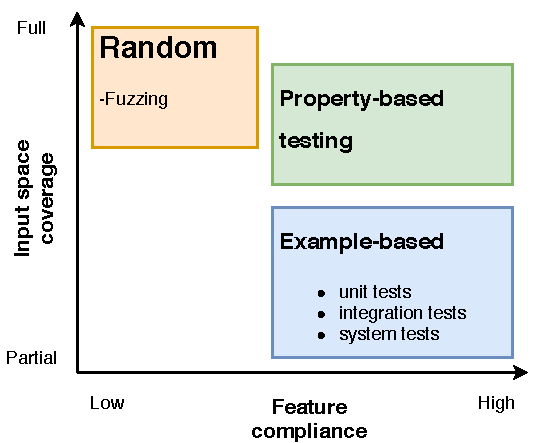
\includegraphics[width=0.7\textwidth]{media/Testing-diagram.pdf}
\end{center}
\caption[A diagram of different automated testing techniques showing input space coverage versus feature compliance]{Testing techniques and their properties.}
\label{fig:testing-techniques-diagram}
\end{figure}
\textbf{Testing of smart contracts.} 
% Due to the potential complexity of interactions between contracts deployed on a blockchain, formal verification in such a setting may prove too difficult. Testing is an ideal alternative approach in this case to discover bugs in contract implementations. As discussed earlier, it may also complement formal verification to identify bugs in contract implementation, or to help uncover mistakes in the formulation of the specification.
 To the authors' knowledge the research field of smart contract testing, in particular \pbt{}, is very sparse at the time of writing. We give a brief overview of existing work in testing of smart contracts. In \cite{contractfuzzing} they develop a fuzzing tool to test contracts on Ethereum. Their tool supports identifying vulnerabilities related to re-entrancy, timestamp dependencies, block number dependencies, potentially unsafe external calls, and gassless calls. Out of 6991 contracts tested, their tool flagged more than 459 vulnerabilities. In particular, it successfully detects the vulnerability of the DAO contract described earlier.

\textit{Echidna} is an open-source smart contract fuzzing tool for Ethereum\cite{echidna}. It is developed in Haskell and uses QuickCheck to support some \pbt{} features such as shrinking and mutation testing, and supports some user-defined testable properties. However the properties seem to be restricted to simple invariants of individual contracts that relate the states between a single execution step of a contract in complete isolation of whatever else might happen on the blockchain.

\textit{Brownie} is a an open-source \pbt{} framework for Ethereum contracts\cite{brownie}. It supports testing \textit{functional} properties of the contract code. For example, given a token contract which uses a function \coq{transfer\_token} to expose a transfer endpoint, Brownie can test assertional properties about \coq{transfer\_token} involving the state of the token contract. It does so by generating a ``random'' blockchain state, and random inputs to the \coq{transfer\_token} function (addresses to transfer between, and number of tokens to send).

These \pbt{} libraries all have in common that they only support testing of functional properties. They do not support temporal properties, nor do they support testing interactions between contracts. As we mentioned with the UniSwap/Lendf.me attack, the vulnerability occurred only in the combination of two interacting contracts. Individually, both contracts were correct. Clearly, existing \pbt{} approaches are insufficient to detect these types of vulnerabilities.
\medskip\\
\textbf{Problem Statement.}
In this thesis we aim to answer study questions:
\begin{itemize}
    \item How can \pbt{} be used to find bugs in smart contracts?
    \item How can we support testing of functional and temporal properties of contracts on realistic data?
    \item How can we test complex interactions between multiple contracts?
    \item How can testing support formal verification of contracts?
\end{itemize}
\textbf{Contributions.} This work contributes with a Coq development of a smart contract \pbt{} framework for \textit{ConCert}, an existing, in-development framework for smart contract verification in Coq. Our framework supports testing of properties on blockchain execution traces. In particular it supports testing of functional and temporal properties on either isolated or interacting contracts. Since the entire development is in Coq, both testing and verification efforts can be combined, and specifications can, to some extend, be shared between testing and verification. We demonstrate the capabilities and limitations of our framework on various case studies. \medskip\\
\textbf{Structure of the thesis.} The remainder of this thesis is structured as follows: in \autoref{ch:quickchick} we give an introduction to QuickChick - Coq's \pbt{} library, and in \autoref{ch:concert} we give an introduction to ConCert, the blockchain and smart contract formalisation in Coq that we base our developments on. In \autoref{ch:design-implementation} we present the design and implementation of our framework, and in \autoref{ch:case-studies} we apply our work in various case studies.

%%%%%%%%%%%%%%%%%%%%%%%%%%%%%%%%%%%%%%%%%%%%%%%%%%%%%%%%%%%%%%%%%%%%%%%

\chapter{Property-Based Testing \& QuickChick}
\label{ch:quickchick}
The purpose of software testing is to increase assurance that a software implementation satisfies a specification. By nature, testing does not give any absolute guarantees, since the behavior is verified against a finite set of test-cases. Therefore it is imperative to employ testing methods that can effectively cover a large subset of the test domain within its inherent finite constraints. In this chapter we give a brief historical perspective on \pbt{} and describe Coq's QuickChick library for \pbt{}, which forms the backbone of our development of testing for smart contracts.
\section{A Brief Historic Perspective}
The term 'Property-Based Testing' was first coined by Fink et al in 1997\cite{fink1997property} as an automated software testing methodology which focuses on formally answering the following key questions:
\begin{itemize}
    \item What is to be accomplished via testing?
    \item What test data should be used?
    \item When has sufficient testing occured?
    \item How is success and failure of a test determined?
\end{itemize}
In the paper, they develop an implementation of the approach using a low-level specification language, TASPEC (Tester's Assistant SPECification language), which automatically translates the specification into a test oracle that will execute the software on generated test data, and verify that the executions satisfy the given property. A simplified overview of the implementation is shown in \autoref{fig:testers-assistant}. One key aspect to note is the level of automation; tests are executed and verified against the specification automatically, without requiring user interference. In contrast, manual software testing approaches require some form of user interaction in order to determine if each test-case\footnote{we use the definition of a test-case as the combination of a program, a property to test on the program, and a concrete input data sample} was successful. Thus, \pbt{} as an idea and methodology marked a significant step forward for software testing.

\begin{figure}[h]
\begin{center}
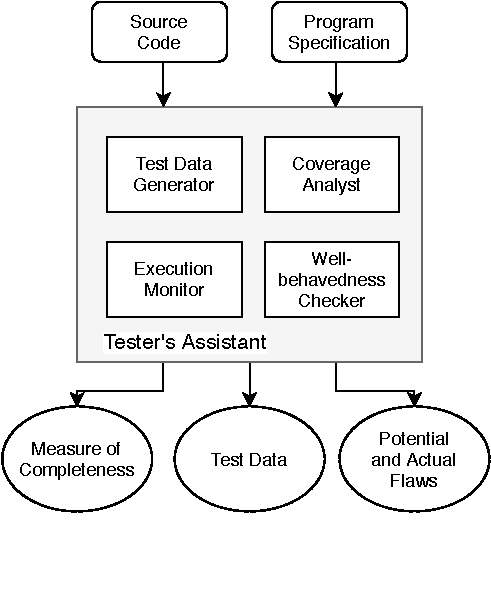
\includegraphics[width=0.6\textwidth]{media/Tester's Assistant.pdf}
\end{center}
\caption[Figure description for the Tester's Assistant from \cite{fink1997property}.]{A simplified overview of the implementation of the Tester's Assistant from \cite{fink1997property}. A source program and a specification is given to the Tester's Assistant, which then tests the program using a test data generator, monitors the test executions, and outputs the various result metrics.}
\label{fig:testers-assistant}
\end{figure}
Since then, \pbt{} has been popularised, in particular in the functional programming community, by Haskell's QuickCheck library\cite{claessen2011quickcheck}, and its approach has become synonymous with \pbt{}. \pbt{} is also sometimes referred to in the literature as Random Property Testing (usually for derivative works of QuickCheck).

\pbt{} has also been employed for proof assistants such as Isabelle\cite{bulwahn2012new} and for Coq in the QuickChick library\cite{denes2014quickchick} (a clone of Haskell's QuickCheck). The authors of QuickChick state that the motivation for using \pbt{} in proof assistants is that experience shows that much time is often spent on trying to prove incorrect statements, and they believe \pbt{} can be combined with the activity of formal verification to reduce the time spent on eventually failed proof attempts, thus reducing the overall cost of formal verification. It is not the primary purpose of this thesis to evaluate this statement, but it is nonetheless an interesting point worth mentioning. In the following section we describe QuickChick in detail and give a few simple, canonical examples of its usage (not related to smart contracts). We use Coq notation for code, but it should be readable by any reader familiar with ML-like languages, Haskell, or any other mainstream functional programming language. We assume the reader is familiar with at least one such language.

\section{QuickChick}
\label{sec:obt-qc}
Although the description we provide here is for Coq's QuickChick library, it can essentially also be seen as a description of Haskell's QuickCheck due to their similarity. For an extended practical introduction to QuickChick with extensive examples we refer to \cite{Pierce:SF4}\footnote{Freely available at \url{https://softwarefoundations.cis.upenn.edu/qc-current/index.html}}. The purpose of this section is to explain the key concepts and code constructs of QuickChick, to provide a basis of understanding for the description of the design and implementation of our smart contract testing framework in \autoref{ch:design-implementation}. Readers familiar with QuickChick or QuickCheck may skip this section.
\medskip\\
Suppose we have implemented a \coq{sort} function for sorting lists of natural numbers in Coq. We want to ensure that this function indeed sorts correctly, meaning it should satisfy the predicate $n_i \le n_{i+1}$ for all adjacent entries in the list. There are many ways to formally state this property. One way is to implement a function, \coq{sorted : list nat -> bool}, that returns true if the given list is sorted and false otherwise. The correctness property on \coq{sort} can then be expressed in Coq as the proposition: (i.e. type)
\begin{code}
\begin{minted}[escapeinside=\\$\\$]{coq}
  forall l, sorted (sort l) = true
\end{minted}
\end{code}
Note that \coq{sorted} is a computable function, and also note that we assume \coq{sorted} is implemented correctly (i.e. it returns true if and only if the list is actually sorted). The latter assumption is one that implicitly always exists when doing any sort of formal verification - namely that the formalised specification in fact correctly describes the desired property. This assumption may of course be wrong - we may have made a mistake in implementing \coq{sorted}, but that is an orthogonal problem to the one we are studying here.

Assume we had a function, \coq{generateNatList : () -> list nat}, that generates a (pseudo-)random list each time it is called. Using this function, it is not hard to imagine how one could create a customized test function of the \coq{sorted} property above that generates, for example, 10.000 random lists and tests that the property above holds for all these lists. If there was an input for which the property did \textit{not} hold, the test function could print or return this counterexample, such that the user could see exactly where it went wrong.

At its core, this is the approach taken by QuickChick, while providing automation for many of the manual steps we had to go through in the \coq{sorted} example; namely everything involving test configuration, counterexample reporting, and even sometimes the generator of input data can be derived automatically. These features are what makes QuickChick an effective and attractive tool for testing. The approach to \pbt{} taken by QuickChick revolves around two key ingredients: a \textit{computable} test property, and generators of ``random'' input data for the function under test. Two less interesting ingredients for our purposes, but equally important, are also: printers and shrinkers. A printer in this context is a function from a type to a string. Any type used in QuickChick must be printable. A shrinker is a function that somehow ``shrinks'' test data. For example, a shrinker for lists could be one that returns all sub-lists of the given list. Shrinkers are used for finding \textit{minimal} counterexamples. When QuickChick finds a counterexample, it will repeatedly shrink the counterexample and re-test the property until it no longer fails. The last ``smallest'' counterexample will be reported by QuickChick. The rationality behind using shrinkers is that it is easier to detect the bug from, say, a list of length 2 than a list of length 100 from visual inspection. Shrinkers are an important part of QuickChick, but they have not been instrumental for our development, so we will not spend much time describing or discussing them. The rest of this section is dedicated to the following components of QuickChick:
\begin{itemize}
    \item The G monad and friends for random data generation
    \item Test Properties and ``checkers''
    \item Automation with Coq's typeclass mechanism
\end{itemize}
After reading this chapter, the reader is encouraged to read \autoref{ch:appendix-qc-example} to see nearly all presented QuickChick features in action on a concrete example.
\subsection{The \coq{G} Monad and Combinators}
The quality of a test is only as good as the quality of the test data. Usually, the larger the test set the better, but size is not the only parameter of quality. When constructing synthetic data, quality can also be measured as how \textit{realistic} it is with respect to the program under test. Similarly, we can also consider the quality of the generating function. A high quality generator for data must not only produce high quality data, it must also produce useful \textit{variation} of data in order to be able to detect e.g. corner cases of the function under test. As an example, a generator for integers that only produces positive numbers may not be of sufficient quality to detect potential bugs when implementing operations on integers,

QuickChick provides several primitives and combinators to support constructing high quality generators. A generator of elements of some type \coq{A} is represented with the type \coq{G A}. In itself, the type constructor \coq{G} of kind \coq{Type -> Type} has no semantic meaning or usefulness. Its meaning is derived from the operators and combinators defined on \coq{G}. All combinators presented in this section are derived, at least in part, from the following two operators on \coq{G}:
\begin{code}
\label{def:returnGen-bindGen}
\begin{minted}[escapeinside=\\$\\$]{coq}
  returnGen : forall (A : Type), A -> G A.
  bindGen   : forall (A B : Type), G A -> (A -> G B) -> G B.
\end{minted}
\end{code}
The first operator, \coq{returnGen}, takes a constant value of some type \coq{A}, and returns a generator which always returns this value. The type signature of \coq{bindGen} might seem obscure at first, but it can simply be seen as a function which takes constructs a generator for elements of type \coq{B} from a generator of elements of type \coq{A} using an intermediate function of type \coq{A -> G B}. Readers familiar with monads will recognize the type signatures of these two functions. Indeed, together they form a monad over \coq{G}. We will not describe monads in detail here. 
For our purposes the benefit of having a monad for \coq{G} is that we can easily introduce the well-known arrow syntax ("\coq{<-}") for chaining multiple calls of \coq{bindGen}. This allows us to write e.g.
\begin{code}
\begin{minted}[escapeinside=\\$\\$]{coq}
  a <- returnGen 42 ;;
  b <- returnGen 9001 ;;
  returnGen (a, b)
\end{minted}
\end{code}
instead of 
\begin{code}
\begin{minted}[escapeinside=\\$\\$]{coq}
  bindGen 
    (returnGen 42)
    (fun a => 
      bindGen
        (returnGen 9001)
        (fun b => returnGen (a, b))
\end{minted}
\end{code}
The former of which is clearly more readable. The above expressions both produce a generator that always returns the pair \coq{(41, 9001)}.
So far we can only generate constants. In order to support non-determinism, QuickChick provides, among others, the following functions:
\begin{code}
\label{def:elems-oneof-freq}
\begin{minted}[escapeinside=\\$\\$]{coq}
  elems_ : A -> list A -> G A.
  oneOf_ : G A -> list (G A) -> G A.
  freq_  : G A -> list (nat * G A) -> G A.
\end{minted}
\end{code}
\coq{elems\_} allows us to sample uniformly at random from a given list. If the list is empty, it will use the given default element. \coq{oneOf\_} is the first generator \textit{combinator} we see aside from \coq{bindGen}. Given a list of generators for elements of type \coq{A}, it will uniformly at random use one of these generators. Similarly to \coq{elems\_}, if the given list is empty, it will return the given default generator. \coq{freq\_} is a variant of \coq{elems\_} where each element in the list is given a relative \coq{weight} to determine the probability of sampling this element. For example, \coq{freq\_ b [(2, x); (3, y)]} will have a 40\% chance of choosing \coq{x}, and a 60\% chance of choosing \coq{y}. 

Note that we do not have to deal with seeds in regards to non-determinism. This is because QuickChick handles seeds internally. Furthermore, a size parameter is hidden in the \coq{G} monad. QuickChick allows manipulation of the size parameter using the functions:
\begin{code}
\label{def:sized-resize}
\begin{minted}[escapeinside=\\$\\$]{coq}
  sized  : (nat -> G A) -> G A.
  resize : nat -> G A -> G A.
\end{minted}
\end{code}
At this point we already have all the tools to construct generators of interesting types. For example, given the following inductive definition of a binary tree:
\begin{code}
\label{def:tree}
\begin{minted}[escapeinside=\\$\\$]{coq}
  Inductive tree A :=
  | leaf : tree A
  | node : A -> tree A -> tree A -> tree A.
\end{minted}
\end{code}
we can easily implement a generator combinator, which returns a generator for \coq{Tree A} of depth \coq{sz}, given a generator for elements of \coq{A}:
\begin{code}
\label{def:genTreeSized}
\begin{minted}[escapeinside=\\$\\$]{coq}
  Fixpoint genTreeSized {A} (sz : nat) (g : G A) : G (Tree A) :=
    match sz with
      | O => returnGen Leaf
      | S sz' =>
          l <- genTreeSized sz' g ;;
          r <- genTreeSized sz' g ;;
          n <- g ;;
          returnGen Node n l r
    end.
\end{minted}
\end{code}
QuickChick provides a large collection of convenient functions and combinators over common data types such as lists, option types, products. We list the most important below for reference, and omit further description. In fact, the behavior of a combinator can usually be inferred solely from its type signature. We encourage the reader to try this on the combinators below. Otherwise, descriptions are available in the \href{https://softwarefoundations.cis.upenn.edu/qc-current/QuickChickInterface.html}{QuickChick Reference Manual}.
\begin{code}
\label{def:listof-vectorof-choose-backtrack-stmaybe-bindgenopt}
\begin{minted}[escapeinside=\\$\\$]{coq}
  listOf    : forall {A : Type}, G A -> G (list A).
  vectorOf  : forall {A : Type}, nat -> G A -> G (list A).
  choose    : forall {A : Type} `{ChoosableFromInterval A},
              (A * A) -> G A.
  backtrack : forall {A : Type}, 
              list (nat * G (option A)) -> G (option A).
  suchThatMaybe :
    forall {A : Type}, G A -> (A -> bool) -> G (option A).
  bindGenOpt : forall {A B : Type},
    G (option A) -> (A -> G (option B)) -> G (option B).
\end{minted}
\end{code}

\subsection{Test Properties \& Checker Combinators}
In the \coq{sort} example we remarked that the \coq{sorted} predicate was computable/decidable, and that this is indeed a necessity for QuickChick and \pbt{} in general. QuickChick formalises this with the \coq{Checkable} typeclass:
\begin{code}
\label{def:checkable}
\begin{minted}[escapeinside=\\$\\$]{coq}
  Class Checkable (A : Type) : Type :=
  {
    checker : A -> Checker
  }.
\end{minted}
\end{code}
where \coq{Checker} is a type that represents the result of a test. A test can either succeed, fail, or be discarded. An instance of the \coq{Checker} typeclass with for some type \coq{A} indicates that we can check the type \coq{A}. For example, the most common instance is for booleans. \coq{false} represents failure, and \coq{true} represents success. Another instance is for the unit type. The unit checker always discards the test.

QuickChick provides various checker combinators that each represent a specific kind of property to check. The most common checker is \coq{forAll}\footnote{Not to be confused with the \coq{forall} type constructor.}, which has the type signature:
\begin{code}
\label{def:forAll}
\begin{minted}[escapeinside=\\$\\$]{coq}
  forAll :
    forall {A prop : Type} 
          `{Checkable prop} 
          `{Show A}
           (gen : G A)
           (pf : A -> prop), Checker.
\end{minted}
\end{code}
This type declaration says that \coq{forAll} is a function that implicitly takes two types, \coq{A} and \coq{prop} where \coq{prop} has a \coq{Checkable} typeclass instance and  \coq{A} has a \coq{Show} instance. Given a generator for \coq{A} and a checkable property \coq{pf} on \coq{A}, this function returns a checker. What this checker represents is that the property \coq{pf} holds for all elements of type \coq{A}. Of course, a test cannot prove that it holds ``for all'' in the mathematical sense. By default, QuickChick will generate 10.000 input samples using \coq{gen}, and verify that \coq{pf} does not fail on any of them. If it does fail, it reports the counterexample. 

Often times one wants to test \textit{conditional} properties. For example, it could be interesting to verify that \coq{forall l, sorted(l) = true -> sort(l) = l}. QuickChick can represent this kind of proposition using the \coq{implication} checker combinator:
\begin{code}
\label{def:implication}
\begin{minted}[escapeinside=\\$\\$]{coq}
  implication :
    forall {prop : Type} 
          `{Checkable prop} 
           (b : bool)
           (p : prop), Checker.
\end{minted}
\end{code}
Note that the ``left-hand side'' of the implication must be a boolean. Whenever \coq{b} is false, the test-case is discarded, and whenever it is true \coq{p} must check successfully. Thus, \coq{implication} almost mimics the logical behavior of implication. QuickChick uses the notation \coq{"x ==> y"} for \coq{implication x y}. We could then define a checker that represents the property above like this:
\begin{code}\begin{minted}[escapeinside=\\$\\$]{coq}
  forAll generateNatList (fun l => sorted(l) ==> sort(l) =? l) 
\end{minted}
\end{code}
where we assume \coq{=?} is notation for boolean equality on lists\footnote{Technically, it does not have to be \textit{boolean} equality - it could be any \coq{Checkable} type. In fact, as we shall see later, it even suffices to be any \coq{Decidable} type}.

Sometimes it might also be useful to test that a property does \textit{not} hold. If the property is stated as a boolean, we can of course just use negation, but since QuickChick prefers to deal with \textit{Checker}s, it comes with a checker combinator that asserts a given input checker \textit{fails} when run:
\begin{code}
\label{def:expectFailure}
\begin{minted}[escapeinside=\\$\\$]{coq}
  expectFailure :
    forall {prop: Type} `{Checkable prop} (p: prop), Checker.
\end{minted}
\end{code}
\coq{(expectFailure p)} will succeed when at least one test of \coq{p} fails. When \coq{(expectFailure p)} succeeds, it will furthermore print the input which made it succeed (i.e. the input that did not satisfy \coq{p}). In an informal way, this combinator models existential quantification in the same way \coq{forAll} models universal quantification. 

QuickChick has several other checker combinators, such as \coq{conjoin} and \coq{disjoin} for conjunction and disjunction of checkers, respectively, and a \coq{collect} combinator which can be used to collect and print various statistics about the execution of a test.


\subsection{Automation with Coq's Typeclass mechanism}
With the tools for generating data and creating checkable properties we have presented so far we can already test complex properties, but it is not very convenient. Checkable properties are terms, while properties used for proofs are propositions (types) in Coq, so we cannot reuse properties between testing and proving yet. Furthermore, we have to keep track of the names of all the generators we use for all different types. Using Coq's typeclass mechanism and its powerful type inference system we can significantly reduce these burdens by automating most of these tasks. QuickChick exposes the following typeclasses for generators:
\begin{code}
\label{def:GenSized-Gen-Shrink}
\begin{minted}[escapeinside=\\$\\$]{coq}
  Class GenSized (A : Type) := { 
    arbitrarySized : nat -> G A 
  }.
  Class Gen (A : Type) := { 
    arbitrary : G A
  }.
  Class Shrink (A : Type) := {
    shrink : A -> list A
  }.
  Class Arbitrary (A : Type) `{Gen A} `{Shrink A}.
\end{minted}
\end{code}
Hierarchically, the typeclasses are related as shown in \autoref{fig:qc-generator-typeclass-hierarchy}. This allows us to write generators more succinctly, and without having to keep track of the names of all our generators. For example, assuming we have \coq{Gen} instances for \coq{nat}s and \coq{bool}s (which QuickChick provides out-of-the-box) we can create a \coq{Gen} instance for \coq{(nat * bool)}\footnote{QuickChick actually already derives \coq{Gen} instances for pairs of any types where it can find a \coq{Gen} instance. Similarly for \coq{Arbitrary}.}  
\begin{code}
\label{def:genNatBoolPair}
\begin{minted}[escapeinside=\\$\\$]{coq}
  Instance genNatBoolPair : Gen (nat * bool) := {
    arbitrary := n <- arbitrary ;;
                 b <- arbitrary ;;
                 returnGen (a, b)
  } 
\end{minted}
\end{code}
Note the use of \coq{arbitrary}. We did not have to specify which generator should be used to produce \coq{n} and \coq{b}. Coq's type inference could guess that the former should be a \coq{nat} and the latter a \coq{bool}. Then Coq looked in its environment for \coq{Gen} instances for those types. For readers with a background in object-oriented programming this can be compared to the use of interfaces, although there are some technical differences.
\medskip\\
QuickChick takes it one step further by exposing a plug-in that uses Coq's meta-programming library MetaCoq to allow for \textit{automatic instance derivation} with the command
\begin{code}
\begin{minted}[escapeinside=\\$\\$]{coq}
  Derive <class> for T
\end{minted}
\end{code}
where \coq{<class>} may be any of \coq{GenSized}, \coq{Shrink}, \coq{Arbitrary}, or \coq{Show}. This means generators can automatically be derived for many types - even inductively defined types. In fact, we could have automatically obtained a generator for \coq{Tree} using \coq{Derive Arbitrary for Tree} with behavior very similar to the one we implemented manually.
\begin{figure}[h]
\begin{center}
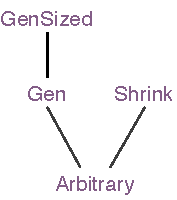
\includegraphics[width=0.2\textwidth]{media/QC Generator Typeclasses Hierarchy.pdf}
\end{center}
\caption[Figure description for the QuickChick Generator Typeclass Hierarchy.]{QuickChick Generator Typeclass Hierarchy. If a type has a \coq{GenSized} instance, it automatically derives a \coq{Gen} instance. If a type has both a \coq{Gen} instance and a \coq{Shrink} instance, it has an \coq{Arbitrary} instance}
\label{fig:qc-generator-typeclass-hierarchy}
\end{figure}
Next we look at how QuickChick connects testable properties (which are Coq functions) and propositions (which are Coq types). To make the issue more clear, we present a simple example with the binary trees we have seen earlier. Suppose we have implemented a \coq{mirror} function on binary trees. We want to assure that \coq{mirror} is an involution, i.e. that \coq{mirror (mirror t) = t}. If we were to \textit{prove} this statement, we could write a lemma in Coq like this:
\begin{code}
\label{def:mirror_is_involution}
\begin{minted}[escapeinside=\\$\\$]{coq}
  Definition mirror_is_involution_P (t : Tree) := 
    mirror (mirror t) = t.
  
  Lemma mirror_is_involution : 
    forall t, mirror_is_involution_P t.
  Proof.
  ...
  Qed.
\end{minted}
\end{code}
Recall that the type of \coq{mirror\_is\_involution} is exactly the proposition we wish to prove, and that discovering a proof of \coq{forall t, mirror (mirror t) = t} is the same as showing that this type is inhabited. Furthermore, note that ``\coq{=}'' denotes Leibniz equality, meaning that it asserts \textit{type} equality. But determining equality of two types is not decidable in general, which is clearly necessary for testing. Then how could we go about testing this proposition in particular? The problem is that we have no computable definition that decides equality of two binary trees. Once again, QuickChick solves this using typeclasses with the \coq{Dec} and \coq{Dec\_Eq} typeclasses:
\begin{code}
\label{def:Dec-Dec_Eq}
\begin{minted}[escapeinside=\\$\\$]{coq}
  Class Dec (P : Prop) : Type := 
  { 
    dec : decidable P 
  }.
  Class Dec_Eq (A : Type) :=
  {
    dec_eq : forall (x y : A), decidable (x = y)
  }.
\end{minted}
\end{code}
where \coq{decidable P} is the proposition \coq{P \textbackslash/ \textasciitilde P}. QuickChick automatically derives \coq{Checkable} instances for all \coq{Dec} instances, so if we implement a decision procedure for equality on our definition of binary trees, then \coq{mirror\_is\_involution\_P} will be decidable and checkable. Consequently, we will be able to use \coq{mirror\_is\_involution\_P} both for testing and proving.
\medskip\\
In this example, there is no difference between the structural equality on trees induced by \coq{=} and a decision procedure for equality on trees (assuming we implemented it correctly), however this is not always the case. For example given a formalisation of propositional formulae with variables, we might consider two formulae equal (or equivalent) up to variable renaming. In this case, we would consider \coq{or a b} and \coq{or c d} equal, but (depending on our representation of variables) the proposition \coq{or a b = or c d} would not be provable in general. This is something to keep in mind when reflecting between the world of terms, and the world of types in Coq. However since it is often the case that the structural equality provided by \coq{=} is indeed the desired notion of equality, QuickChick provides a tactic, \coq{dec\_eq}, that can automatically derive decidable instances of equality on many user-defined types by using structural equality.

In summary, QuickChick provides many automation tools to make testing development easier, faster, and more flexible, and it provides mechanisms for connecting testing and proving efforts. To see QuickChick in action on a concrete example, we refer to \autoref{ch:appendix-qc-example} where we use QuickChick to test confluence of the untyped lambda calculus. We highly recommend readers previously unfamiliar with QuickChick or QuickCheck to read this chapter.

%%%%%%%%%%%%%%%%%%%%%%%%%%%%%%%%%%%%%%%%%%%%%%%%%%%%%%%%%%%%%%%%%%%%%%%

\chapter{ConCert - A Blockchain Formalisation \& Smart Contract Execution Framework in Coq}
\label{ch:concert}
\href{https://github.com/AU-COBRA/ConCert}{\cc{}} is a blockchain formalisation\cite{DBLP:journals/corr/abs-1907-10674} and smart contract execution framework\cite{nielsen2019smart} in Coq. It is developed by the \href{https://concordium.com/}{Concordium Blockchain Research Center} at Aarhus University and is under active development at the time of writing.

The aim of \cc{} is to support certified blockchain and smart contract development in a manner where both the blockchain formalisation, a Coq embedding of the smart contract language, and concrete contract implementations can be formally verified in the same framework. Key soundness theorems connect these different representations. Ongoing developments aim to also provide support for certified extraction to existing smart contract languages such as Tezos' Liquidity or Michelson. In this work we interact almost exclusively with the execution framework in \cc{} since our goal is to test execution of concrete contracts. Therefore the focus focus will be on describing this part of \cc{}. A full presentation and overview of \cc{} can be found in the original paper\cite{DBLP:journals/corr/abs-1907-10674}.

The rest of this chapter is structured as follows: in \autoref{sec:execution-framework} we describe the implementation of the execution framework. In particular we describe different execution models, and key type definitions that will be important in describing our testing framework in \autoref{ch:design-implementation} and subsequent case studies. In \autoref{sec:erc20-example} we give an example of a \cc{} contract implementing the ERC-20 specification for tokens.

\section{The Execution Framework}
\label{sec:execution-framework}
Smart contracts are programs executed on a blockchain. They modify the state of the blockchain by performing transactions or interacting with other deployed contracts. Contracts may themselves also have local states, which are stored on the blockchain. When developing a smart contract language and an execution model there are some key questions which should be considered:
\begin{itemize}
    \item How, which, and when are contracts allowed to modify contract states?
    \item How do contracts interact?
    \item How will the execution layer schedule calls between contracts?
\end{itemize}
\cc{} uses Coq's embedded functional language Gallina to model contracts. This means contracts in \cc{} are Coq terms. As an important side benefit, this allows us to also utilize Coq's extensive library ecosystem and use formally verified software to develop contracts, and it allows us to even formally verify functional properties of the contracts in complete isolation from the execution layer.
To model execution of smart contracts, certain base operations about how contracts and accounts are identified. \cc{} uses a Coq typeclass to represent this:
\begin{code}
\label{def:chainbase}
\begin{minted}[escapeinside=\\$\\$]{coq}
  Class ChainBase := {
    Address : Type;
    address_eqb : Address -> Address -> bool;
    address_eqb_spec :
      forall (a b : Address), Bool.reflect (a = b) (address_eqb a b);
    address_eqdec :> stdpp.base.EqDecision Address;
    address_countable :> countable.Countable Address;
    address_serializable :> Serializable Address;
    address_is_contract : Address -> bool;
  }.
\end{minted}
\end{code}
This says that an \coq{Address} is some type that is countable, comparable for equality, serializable (we will explain what this means further down) and has a predicate function for identifying whether the address refers to a contract (if it does not refer to a contract, it is assumed to refer to an account instead). In the following definitions we assume an instance of this class is present. A simple example instance, which is indeed the one we use in our testing framework, is where \coq{Address} is a bounded natural number with some bound $N$ where addresses from $N/2$ to $N$ are identified as contract addresses, and the rest are identified as account addresses.

In \cc{} contracts interact using a message passing paradigm. To support user-defined message types it uses a serialization/de-serialization technique by requiring that messages being sent must implement a \coq{Serializable} typeclass
\begin{code}
\label{def:SerializedValue-Serializable}
\begin{minted}[escapeinside=\\$\\$]{coq}
  Record SerializedValue := {
    ser_value_type : SerializedType;
    ser_value : interp_type ser_value_type;
  }.
  
  Class Serializable (ty : Type) := {
    serialize : ty -> SerializedValue;
    deserialize : SerializedValue -> option ty;
    deserialize_serialize x : deserialize (serialize x) = Some x;
  }.
\end{minted}
\end{code}
\newcommand{\serializable}{\hyperref[def:SerializedValue-Serializable]{\coq{Serializable}}}
\newcommand{\serializedValue}{\hyperref[def:SerializedValue-Serializable]{\coq{SerializedValue}}}
where \serializedValue{} is a record that contains serialized representation of the type, and the value itself in the serialized format. The \serializable{} typeclass requires that the composition of de-serialization and serialization  is essentially the identity function for elements of the given type \coq{ty}. \cc{} provides \serializable{} instances for many common types such as natural numbers, bounded numbers, booleans, sum types, product types, lists, maps, sets, optional types, ect. (assuming that any parametric types also have \serializable{} parameters). It also provides automation for deriving \serializable{} instances for non-recursive, inductively defined types.

Contracts need to access and interact with the blockchain, but they need not know of all the internal details blockchain. In particular, contracts should not be able to access the local states of other contracts. The blockchain view exposed to contracts is defined with the \coq{Chain} type:
\begin{code}
\label{def:Amount}
\begin{minted}[escapeinside=\\$\\$]{coq}
  Definition Amount := Z.
  Record Chain := {
    chain_height : nat;
    current_slot : nat;
    finalized_height : nat;
    account_balance : Address -> Amount;
  }.
\end{minted}
\end{code}
When contracts are called, they need to some contextual information such as the address of the caller, and if the call carries money (the asset of the blockchain). This is gathered in the \coq{ContractCallContext} type:
\begin{code}
\label{def:ContractCallContext}
\begin{minted}[escapeinside=\\$\\$]{coq}
  Record ContractCallContext := {
    ctx_from : Address;
    ctx_contract_address : Address;
    ctx_amount : Amount;
  }.
\end{minted}
\end{code}
\cc{} employs a functional approach in its representation of contracts, as well as how contracts modify their local states. The executable part of a contract is essentially just a function from a message type and a current state to a new state and a list of actions (transfers, calls to other contracts, or deployment of a new contract). This is captured by the \coq{Contract} type 
\begin{code}
\label{def:Contract}
\begin{minted}[escapeinside=\\$\\$]{coq}
  Record Contract
      (Setup Msg State : Type)
      `{Serializable Setup}
      `{Serializable Msg}
      `{Serializable State} :=
  build_contract {
    init :
      Chain ->
      ContractCallContext ->
      Setup ->
      option State;
    receive :
      Chain ->
      ContractCallContext ->
      State ->
      option Msg ->
      option (State * list ActionBody);
  ...
  }.
\end{minted}
\end{code}
In other words, a contract consists of an initialisation function, which constructs an initial state from a setup, and a receiver function which receives a message and returns a new state and a list of actions to be performed after its state has been updated. The execution is allowed to fail. This occurs when \coq{receive} returns \coq{None}. The actual definition of \coq{Contract} in the source code of \cc{} contains a few more fields which require that \coq{init} and \coq{receive} respect an equivalence relation on the \coq{Chain} type, namely the relation that two chains are equivalent if they are extensionally equal\footnote{If functional extensionality ($\forall x, y, f, g: f(x) = g(x) \rightarrow f = g$) is assumed then the equivalence becomes equality}.
\medskip\\
\textbf{Semantics of the execution layer}. 
The \coq{Chain} type presented earlier is only the contracts' view of the blockchain and does not contain the necessary information for execution of actions. The \coq{Environment} type extends \coq{Chain} with information about currently deployed contracts and their local states. From this we can implement an evaluation procedure for a single action (a transfer, contract call, or a contract deployment) which outputs an updated environment along with a list of new actions to evaluate. This is done in a fairly straightforward way, so we omit any formal description. As an example, evaluation of a transfer requires that the sending address has sufficient balance. In the resulting \coq{Environment} the account balances are updated accordingly. No new actions are emitted.
\newcommand{\evalto}{\mathrel{\Downarrow}}
\newcommand{\eval}[4]{\langle #1, #2 \rangle \evalto (#3, #4)}
\newcommand{\stepto}{\rightarrow}
\newcommand{\step}[2]{#1 \stepto #2}
\newcommand{\reachto}{\mathrel{\rightarrow^*}}
\newcommand{\reachable}[2]{#1 \reachto #2}
\newcommand{\traceto}[1][\pi]{\xrightarrow{#1}\mathrel{\vphantom{\to}^*}}
\newcommand{\trace}[3][\pi]{#2 \traceto[#1] #3}
\newcommand{\nil}{\texttt{[]}}
\newcommand{\cons}{\mathbin{::}}
\newcommand{\app}{\mathbin{++}}
\newcommand{\Perm}{\text{Perm}}

%\newcommand{\eval}[3]{$\langle #1, #2 \rangle \Downarrow (#1', #3)$}
\newcommand{\cstep}[4]{(#1, #2) \rightarrow (#3, #4)}
Next we define what it means for the blockchain to take a ``step''. First, let $\eval{\sigma}{a}{\sigma'}{l}$ be evaluation of the action $a$ under the environment $\sigma$, with resulting environment $\sigma'$ and emitted list of actions $l$. Furthermore let $\cstep{\sigma}{l}{\sigma'}{l'}$ denote a valid step of the blockchain where $\sigma$ is an environment and $l$ is a list of actions. We give the small-step semantics of $\rightarrow$ below\footnote{The inference rules are taken from \cite{nielsen2019smart} and are used with permission from the authors.}. 
\begin{figure}[h]
\begin{mathpar}
  \infer[step-block]
  { b \ \text{valid for} \ \sigma \\ acts \ \text{from accounts} }
  { \step{(\sigma, \nil)}{(\texttt{add\_block}\ b\ \sigma, acts)} }
  \and
  \infer[step-action]
  { \eval{\sigma}{a}{\sigma'}{l} }
  { \step{(\sigma, a \cons l')}{(\sigma', l \app l')} }
  \and
  \infer[step-permute]
  { \Perm(l, l') }
  { \step{(\sigma, l)}{(\sigma, l')} }
\end{mathpar}
\end{figure}
The \textsc{step-block} rule states that adding a new block with a list of actions $acts$ to the chain, when the previous chain state has no outstanding actions to be evaluated, is a valid step if the new block $b$ is valid w.r.t the previous environment $\sigma$, and all the actions are from accounts, i.e. from non-contract addresses. Note that \coq{add\_block} is a Coq function that actually \textit{computes} the new environment. The \textsc{step-action} rule formalises how evaluation of the first action in the queue updates the environment. Note that any new actions returned by evaluation of $a$ are inserted \textit{before} existing list of actions to be evaluated. This models a depth-first execution order. To allow different execution orders, the \textsc{step-permute} allows permutations of the queue of actions to be evaluated. For example, it is possible to emulate a breadth-first execution order by performing a \textsc{step-permute} after every \textsc{step-action} with the particular permutation that appends the new actions at the bottom of the queue. In this case the queue behaves like a FIFO queue. The step relation naturally generalises to entire execution \textit{traces} as the transitive closure of $\rightarrow$.


\section{An Example: An Implementation of the ERC-20 Token Standard}
\label{sec:erc20-example}
Tokens are commonly used in smart contracts to represent some transferable asset. There exists many standards but perhaps the most well known is the ERC-20 Token Standard. In this example we present an implementation of a specific instance from the Ethereum blockchain named EIP-20\cite{eip20}. Our implementation in \cc{} is essentially a port of \href{https://github.com/ConsenSys/Tokens/blob/fdf687c69d998266a95f15216b1955a4965a0a6d/contracts/eip20/EIP-20.sol}{ConsenSys's implementation}. The full source code is available in the \href{https://github.com/AU-COBRA/ConCert/blob/master/execution/examples/EIP-20Token.v}{\cc{} Github repository}.
\medskip\\
In short, the EIP-20 Token contract supports three actions: transfers between accounts, transfers on behalf of accounts, and approvals of transfers on behalf of the calling account. We represent these actions in the \coq{Msg} type of the contract
\begin{code}
\label{def:EIP20-TokenValue}
\begin{minted}[escapeinside=\\$\\$]{coq}
  Definition TokenValue := N.
  Inductive Msg :=
  | transfer : Address -> TokenValue -> Msg
  | transfer_from : Address -> Address -> TokenValue -> Msg
  | approve : Address -> TokenValue -> Msg.
\end{minted}
\end{code}
\coq{transfer addr n} transfers \coq{n} tokens to \coq{addr} from the calling address. The action should fail whenever the caller's token balance is less than \coq{n}. It is the responsibility of the contract to keep track of this information. \coq{transfer\_from from to n} transfers \coq{n} tokens from \coq{from} to \coq{to}, assuming \coq{from} has already approved the caller to transfer at least \coq{n} tokens on its behalf. After a \coq{transfer\_from} action has been successfully executed, the allowance should be updated correspondingly. It is also the responsibility of the token contract to keep track of all this information. Finally, in \coq{approve addr n} the caller approves \coq{addr} to transfer up to \coq{n} tokens on its behalf. The contract keeps track of this information with the following definition of its \texttt{State}:
\begin{code}
\label{def:EIP20-State}
\begin{minted}[escapeinside=\\$\\$]{coq}
  Record State := {
    total_supply : TokenValue;
    balances : FMap Address TokenValue;
    allowances : FMap Address (FMap Address TokenValue)
  }.
\end{minted}
\end{code}
The \coq{allowances} maps from an allower address to a map containing all the addresses allowed to transfer on the allowers behalf, and how many tokens they are allowed to transfer. 
Initially, the owner of the contract is given a specified number of tokens:
\begin{code}
\label{def:EIP20-Setup}
\begin{minted}[escapeinside=\\$\\$||]{coq}
  Record Setup := {
    owner : Address;
    init_amount : TokenValue;
  }.
  Definition init (chain : Chain)
	              (ctx : ContractCallContext)
	              (setup : Setup) : option State :=
    Some {| 
      total_supply := setup.(init_amount);
      balances := 
        FMap.add setup.(owner) setup.(init_amount) FMap.empty;
      allowances := FMap.empty
    |}.

\end{minted}
\end{code}
The \coq{receive} function of the contract becomes:
\begin{code}
\label{def:EIP20-receive}
\begin{minted}[escapeinside=\\$\\$]{coq}
  Definition receive (chain : Chain)
	                 (ctx : ContractCallContext)
	                 (state : State)
	                 (maybe_msg : option Msg)
        : option (State * list ActionBody) :=
    let sender := ctx.(ctx_from) in
    let without_actions := option_map 
        (fun new_state => (new_state, [])) in
    (* Only allow calls with no money attached *)
    if ctx.(ctx_amount) >? 0
    then None
    else match maybe_msg with
    | Some (transfer to amount) => 
      without_actions (try_transfer sender to amount state)
    | Some (transfer_from from to amount) =>
      without_actions (try_transfer_from sender from to amount state)
    | Some (approve delegate amount) => 
      without_actions (try_approve sender delegate amount state)
      (* Any other type of message is not allowed.
	     In particular, transfer actions to this 
	     contract are not allowed *)
    | None => None
    end.
\end{minted}
\end{code}
Where \coq{try\_transfer}, \coq{try\_transfer\_from}, and \coq{try\_approve} are functions that perform the access controls and state updates according to the informal description we gave earlier so we omit their implementations.

We have omitted some boilerplate code such as deriving \serializable{} instances for \coq{Setup}, \coq{State}, and \coq{Msg}, and proofs that \coq{init} and \coq{receive} respect the chain equivalence relation that we discussed earlier. \cc{} provides tactics to automate these proofs, so no almost no effort is to obtain an instance of the \coq{Contract} typeclass. In \autoref{sec:erc20-case-study} we test our implementation against the EIP-20/ERC-20 specifications.

%%%%%%%%%%%%%%%%%%%%%%%%%%%%%%%%%%%%%%%%%%%%%%%%%%%%%%%%%%%%%%%%%%%%%%%


\chapter{Design \& Implementation of the Testing Framework}
\label{ch:design-implementation}
This chapter assumes that the reader has read \autoref{ch:quickchick} and \ref{ch:concert}. The goal of our development is to support \pbt{} of smart contracts in ConCert using Coq's QuickChick. There are three questions we must answer to decide on a design of such a system:
\begin{itemize}
    \item What is a suitable, \textit{executable} representation of valid blockchain execution traces?
    \item How can we generate sufficiently ``random'' valid transactions/contract calls using QuickChick's tools?
    \item How can we represent functional properties of contracts and temporal properties on potentially multiple interacting contracts, and how can we manifest these properties as checkable functions over traces?
\end{itemize}
 
\section{Design}
\textbf{Representation of execution traces.} We begin by examining how traces can be represented. Recall from \autoref{ch:concert} that the \coq{add\_block} Coq function is key to what makes ConCert's formalisation of the execution framework \textit{executable}. The executable part of \coq{add\_block} is implemented in the function \coq{add\_block\_exec}. It has the type signature:
\begin{code}
\label{def:add-block-exec}
\begin{minted}[escapeinside=\\$\\$]{coq}
  add_block_exec : bool -> 
                   LocalChain -> 
                   BlockHeader -> 
                   list Action -> option LocalChain.
\end{minted}
\end{code}
An \coq{Action} in ConCert represents anything that can be sent between accounts and contracts on the blockchain. This can either be a monetary transaction between accounts or contracts, a call to a contract, or a call to deploy a contract. The boolean argument denotes whether execution should be depth-first (\coq{true}) or breadth-first (\coq{false}). The \coq{LocalChain} is the concrete blockchain type we operate on, which is an instance of the \coq{Chain} typeclass that represents the state of the blockchain. The \coq{BlockHeader} argument contains information about the new block to be added (block height, block slot number, creator, finalization reward, etc.), and finally a list of \coq{Action}s (messages) that should be executed in the new block. If execution succeeds, it returns a new blockchain state, and otherwise returns \coq{None}. We can use \coq{add\_block\_exec} to act as one ``step'' of execution in a trace. A valid trace then simply becomes a sequence of repeated applications of \coq{add\_block\_exec} from some initial \coq{LocalChain}.
\medskip\\
\textbf{Generators for actions}. For each step, we also need to somehow generate a list of \coq{Action}s to execute in that block, otherwise the execution traces is just a list of empty blocks. The actions we are interested in appearing in generated execution traces depend on which contracts are deployed to the chain. For example, suppose we want to test the EIP-20/ERC-20 Token contract described earlier in \autoref{ch:concert}, and suppose it has been deployed on the chain. Generated execution traces should then contain calls to endpoints of this contract, i.e. we require a generator of \coq{Action}s containing either \coq{transfer}, \coq{transfer\_from}, or \coq{approve} messages. However, if these messages are generated entirely at random they are unlikely to be valid, let alone useful for testing. For example, a valid \coq{(transfer from to nr\_tokens)} requires that the owner of the transfer has enough tokens to transfer, and a valid \coq{(transfer\_from caller from to nr\_tokens)} requires that the owner has approved the caller to transfer enough tokens on its behalf. If they are generated at random it is highly unlikely that execution succeeds, and so most data will be discarded for testing. For more complex contracts this probability may be even smaller. Clearly, if we want testing to be effective, the generator for actions to be executed on the chain must be specialized to adhere, at least partially, to some form of validity requirements with respect to the deployed contracts on the blockchain.

This leads to a central discussion about entirely random input generators versus specialized input generators. As summarized in \autoref{fig:generators-vs}, completely random input generators have low probability of satisfying some arbitrary property $P$, whereas a specialized/customized generator specifically designed to generate input satisfying $P$ will naturally have a higher probability. The specialized generator is more performant in testing since less test data will be discarded. However, a downside of specialized generators is that they require much more user effort, whereas a completely random generator can often be automatically derived for almost any type, and indeed QuickChick provides automation for deriving these kinds of random generators. Another downside of specialized generators is that during implementation, the programmer may (either consciously or not) under-approximate the set of inputs satisfying $P$ in order to simplify implementation efforts or reduce complexity of the generator. This leads to a lesser degree of input space coverage which reduces overall test quality, thus reducing the bug-finding effectiveness of subsequent any test using this generator. One has to keep in mind these things when doing \pbt{} in any domain, and it usually a case-by-case analysis to decide which approach is best. Sometimes it is acceptable to sacrifice some performance in order to reduce implementation efforts or improve input space coverage, or vice versa.

\begin{figure}[h]
\begin{center}
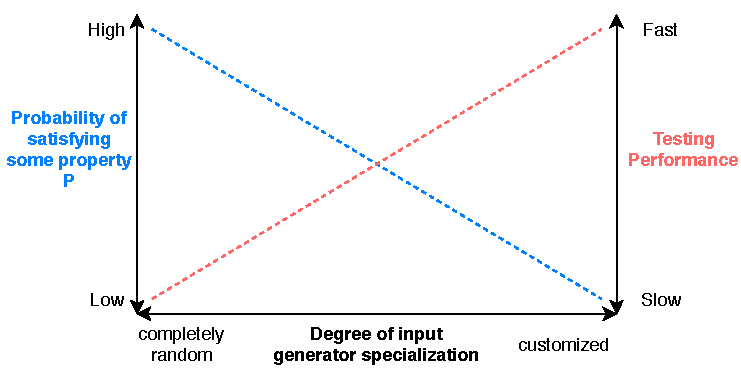
\includegraphics[width=0.9\textwidth]{media/random-vs-specialized-generators.pdf}
\end{center}
\caption[A diagram showing the benefits downsides when either specializing a generator, or generalizing it.]{Properties of random versus specialized input generators.}
\label{fig:generators-vs}
\end{figure}
As discussed earlier in the ERC-20 example, in our case of testing smart contracts we need specialized generators for generating (mostly) valid contract calls. We therefore choose to sacrifice a potential area of automation, and accept that we may slightly under-approximate the set of valid execution traces in order to gain the necessary performance. This means that the user must supply implementations of message generators for the contracts they wish to test. A key usability goal of our development is to provide the user with sufficient tools to easen the implementation efforts of these generators. In our case studies in \autoref{ch:case-studies} we demonstrate how to implement these generators. Luckily, this something that needs to be done only once per contract and, as we shall see later, these generators compose nicely.
% This choice is derived from a few preliminary examinations using entirely random input generators for the ERC-20 token contract, which showed that nearly no valid execution traces were ever generated, and since this contract is very simple compared to other contracts we test in \autoref{ch:case-studies}, we concluded specialized generators were necessary.
\medskip\\
\textbf{Testable properties over execution traces}. The properties we wish to test are summarized in \autoref{fig:testable-props}, along with their approximation/interpretation as executable and testable functions over traces. The first one asserts universal quantification over traces. This definition is general enough to support almost any property. $P$ could be a property on the steps, or on the chain state of each step, or on the state of a specific contract deployed on the chain at each step. The testable interpretation is straightforward: simply generate many traces and test that $P$ holds on each of them. This can be implemented in QuickChick using the \coq{forAll} checker. \medskip\\
The second property deals with reachability. We don't formalise the notion of reachability of a chain state $c$, but intuitively it just means there exists a sequence of steps that ends in $c$. QuickChick has no built-in checker that models existential quantification, but we can approximate it by using the tautology $\exists x, \ P \Rightarrow \neg \forall x, \ \neg P$. With this, testing for existence becomes asserting failure on the assertion that $\neg P$ always holds. \medskip\\
In the third property we use Hoare-triple notation to state a pre-post condition property on a contract, given some incoming message. We use this to test functional properties on contracts. The testable approximation involves generating traces, and checking for each step if the contract $C$ is deployed on the chain, and if there is an \coq{Action} to be executed in this step whose message satisfies $P$. If so, then executing the contract's \coq{receive} function should result in a new contract state satisfying $Q$. Note that all the testable interpretations rely on generating traces. Next we look at how we implemented the design choices presented in this section.
\begin{table}[h]
\centering
\begin{tabular}{ |c|c|c| } 
\hline
Property & Testable interpretation \\
\hline
$\forall t : Trace, \ P(t)$ & \multirow{2}{16em}{generate multiple (e.g. 10.000) traces and test $P$ on each} \\
&\\ %empty row
\hline
$\exists c : Chain, \ reachable(c) \land P(c)$ & \multirow{4}{16em}{generate multiple traces and assert that the test of $\neg P(c)$ fails in some step of a trace. Print counterexample as witness of $P(c)$} \\
&\\&\\&\\ %three empty rows
\hline
\multirow{3}{14em}{Given a contract $C$, \\$\forall m : Msg,$\\$ \{P(C,m)\}C.\coq{receive}(m)\{Q(C,m)\}$} & \multirow{4}{16em}{generate multiple traces and check for each step if there are messages to $C$ satisfying $P$. If so, execute $C.$\coq{receive} and check if $Q$ holds.}  \\
&\\&\\&\\
\hline
\end{tabular}
\caption{Properties over execution traces, and their testable interpretations.}
\label{fig:testable-props}
\end{table}

\newpage
\section{Implementation}
In this section we present key parts of our implementation. This involves generators for traces, and QuickChick \coq{Checker}s that implement the testable interpretation of the properties stated in \autoref{fig:testable-props}. We have simplified some of the example code presented in this section to make presentation easier. We refer to the source code for further details. The source code is available on our \href{https://github.com/mikkelmilo/ConCert}{Github repository}, which is a fork of the \href{https://github.com/AU-COBRA/ConCert}{official ConCert repository}.

An overview of the structure of our testing framework is shown in \autoref{fig:testing-framework-overview}. The user supplies an initial blockchain setup which consists of an initial mapping of accounts and their balances, and a list of contracts to be deployed initially on the chain. The user also supplies QuickChick generators for \coq{Action}s of the deployed contracts. Of course, the user must also supply the property to test on the generated chains. As an aside, QuickChick requires \coq{Show} instances (string representations) for all types used for testing. These are often trivial to implement, or can be derived automatically, so we will not discuss these further. The framework builds a trace generator from the chain setup and \coq{Action} generators. This generator is used by QuickChick to supply test data for the test property, and finally QuickChick outputs a result, either indicating all tests passed, or it prints a specific counterexample that violated the test property.  
\begin{figure}[h]
\begin{center}
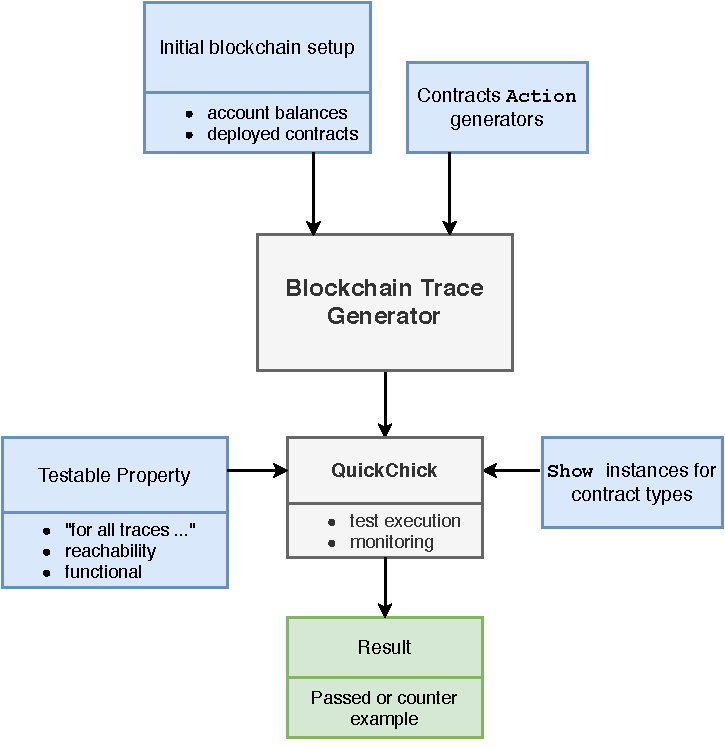
\includegraphics[width=0.8\textwidth]{media/testing-framework.pdf}
\end{center}
\caption[Testing framework structure.]{Testing framework structure. Blue shaded boxes indicate what the user must supply.}
\label{fig:testing-framework-overview}
\end{figure}
\medskip\\
\textbf{Traces}. As previously discussed, we use \coq{add\_block\_exec} to act as one step in an execution trace. We formalise this notion of a step and a trace in Coq with the types:
\begin{code}
\label{def:LocalChainStep}
\begin{minted}[escapeinside=\\$\\$]{coq}
  Inductive LocalChainStep : Type :=
  | step_action : forall (prev_chain : LocalChain) 
                         (header : BlockHeader) 
                         (next_chain : LocalChain) 
                         (acts : list Action), 
                         LocalChainStep.
                         
  Definition LocalChainTraceList := list LocalChainStep.
\end{minted}
\end{code}
\coq{LocalChainStep} is a type with a single constructor, \coq{step\_action}, which takes a previous chain state, a header, a new chain state, and a list of actions. A trace on these steps is just a list of \coq{LocalChainStep}. Note that these definitions say nothing about how we compute the next chain state, but as we will see later, we will construct \coq{LocalChainStep}s such that
\begin{code}
\begin{minted}[escapeinside=\\$\\$]{coq}
  add_block_exec depth_first_param prev_chain header acts 
  = Some next_chain
\end{minted}
\end{code}
intuitively always holds for any generated step\footnote{We have not \textit{proved} that this holds, but by construction it is intuitive that it should be true.}. In other words, this ensures that the step is valid according to \coq{add\_block\_exec}. Similarly, we connect steps in \coq{LocalChainTraceList} by ensuring in the trace generator that for any two adjacent steps indexed by \coq{i} and \coq{i+1}, informally it will hold that 
\begin{code}\begin{minted}[escapeinside=\\$\\$]{coq}
  next_chain_i = prev_chain_(i+1)
\end{minted}
\end{code}
This means there is some duplication of information held in these steps, but it is convenient for testing since it allows us to inspect and compare adjacent chain states in a trace from a single step without having to access the adjacent steps. When we define concrete properties to test in our case studies in \autoref{ch:case-studies} we will utilize this convenience.

Next we look at how to implement a generator for valid traces. Since we have chosen to delegate generation of actions containing contract calls to the user of the framework, the trace generator should be parameterised with some \coq{Action} generator. The behavior of the generator should be as follows: Given some initial chain state, generate a list of ``random'' actions. Use \coq{add\_block\_exec} to add and execute a new block with these actions. If execution succeeds (i.e. \coq{add\_block\_exec} returns a new chain state), then we have a successful ``step''. Repeat this procedure on the new chain state until either no actions could be generated, or \coq{add\_block\_exec} fails, or we have reached a maximum length of the trace. A simplified version of the implementation is shown below. Some notes about the functions used below:
\begin{itemize}
    \item \coq{optToVector} takes a generator of type \coq{G (option A)}, samples it $n$ times and discards any \coq{None} values.
    \item \coq{mk\_basic\_step\_action} calls \coq{add\_block\_exec} with some fixed way of computing block headers and returns a \coq{LocalChainStep} and a \coq{LocalChain} (the new chain state). 
\end{itemize}
\begin{code}
\label{def:gLocalChainTraceList_fix}
\begin{minted}[escapeinside=\\$\\$]{coq}
  Fixpoint gLocalChainTraceList_fix 
    (prev_lc : LocalChain)
    (gActOptFromLCSized : LocalChain -> G (option Action))
    (length : nat)
    (max_nr_acts_per_block : nat) 
    : G LocalChainTraceList :=
  match length with
  | 0 => returnGen []
  | S length => 
    (* sample up to max_nr_acts_per_block actions *)
    acts <- optToVector max_nr_acts_per_block 
                        (gActOptFromLCSized prev_lc) ;;
    lc_opt <- 
      if 0 <? (List.length acts)
      (* compute step and new chain *)
      then returnGen (mk_basic_step_action prev_lc acts)
      else returnGen None ;;
    match lc_opt with
    | Some (lc, step) => 
      (* recurse and append result to this step *)  
      trace <- gLocalChainTraceList_fix lc 
                                        gActOptFromLCSized 
                                        length 
                                        max_nr_acts_per_block ;;
      returnGen (step :: trace)
    | None => returnGen []
    end
  end.
\end{minted}
\end{code}
\textbf{Checkers}. Next, we present the checkers that implement the testable properties described earlier that we wish to support in our framework. 

The implementation of \coq{forAllTraces} is shown below. It takes maximal length parameter, an initial chain from which the trace should start at, a function \coq{gTrace} which generates traces up to some size, and finally it takes a testable property, \coq{pf}, on the chain. This function can return any type as long as it is \coq{Checkable}. For instance, it could be a boolean predicate. Given these arguments, the implementation is rather straightforward: we use QuickChick's \coq{forAll} combinator to generate traces using \coq{gTrace}, and assert that the \coq{next\_chain} of each step satisfies the predicate \coq{pf}. There is only the special case in which the trace is empty. This should not cause the test to fail, since \coq{pf} is trivially satisfied. We use a common ``hack'' to tell QuickChick that this case should be considered a \textit{discarded} test case by using the \coq{false ==> true} checker. Whenever QuickChick sees this, it discards the test. This is useful also when gathering test statistics. Some notes about the functions/notations used:
\begin{itemize}
    \item recall \coq{forAll}'s (simplified) type signature: \coq{(G A) -> (A -> prop) -> Checker}
    \item \coq{next\_lc\_of\_lcstep} is a helper function that retrieves the \coq{next\_chain} field of a \coq{step\_action} 
    \item \coq{false ==> true} and \coq{conjoin} were introduced in \autoref{sec:obt-qc}
    \item \coq{o} is notation for function composition, i.e. \coq{f o g := fun x => f(g(x))}
    \item \coq{checker} turns a an element of a \coq{Checkable} type into a \coq{Checker}, i.e. something that succeeds, fails, or is discarded. 
\end{itemize}
\begin{code}
\label{def:forAllTraces}
\begin{minted}[escapeinside=\\$\\$]{coq}
  Definition forAllTraces 
    (maxLength : nat)
    (init_lc : LocalChain)
    (gTrace : LocalChain -> nat -> G LocalChainTraceList)
    {prop : Type}
   `{Checkable prop}
    (pf : LocalChain -> prop) : Checker :=
  forAll (gTrace init_lc maxLength) 
    (fun trace => 
      match trace with
      | [] => false ==> true
      | _ => conjoin (map (checker o pf o next_lc_of_lcstep) trace)
      end). 
\end{minted}
\end{code}
Next we look at how to define reachability. Since reachability uses existential quantification, we first implement a \coq{Checker} that implements a testable notion of existential quantification. Note that this is a sound but not complete representation of existential quantification in the sense that, if it finds a witness it should indeed be a valid witness, but it may fail to find a witness even though there exists one. This is of course a fundamental limitation of testing that we cannot change, but it is worth keeping in mind. Note that unlike in \coq{forAllTraces}, the property function \coq{p} must be a boolean predicate such that we can negate the property. This limits the set of possible, testable properties we can state using \coq{existsP}, but it is unavoidable. With \coq{existsP}, it is easy to define a reachability checker by asserting that there exists a trace where \coq{pf} holds in at least one step. If we specialize \coq{reachableFromSized} to a specific trace generator and max length, we can introduce a convenient notation \coq{lc \textasciitilde\textasciitilde> pf} in place of \coq{(reachableFromSized \_ lc \_ pf)} to denote the assertion that a state satisfying \coq{pf} is reachable from an initial state \coq{lc}.
\begin{code}
\label{def:existsP-reachableFromSized}
\begin{minted}[escapeinside=\\$\\$]{coq}
  Definition existsP
    {A prop : Type} 
   `{Checkable prop} 
    (g : G A) 
    (p : A -> bool) := 
  expectFailure (forAll g (fun a => negb (p a))).
    
  Definition reachableFromSized
    (maxLength : nat) 
    (init_lc : LocalChain)
    (gTrace : (LocalChain) -> nat -> G LocalChainTraceList)
    (pf : LocalChainStep -> bool)
    : Checker := 
  existsP (gTrace init_lc maxLength) (fun trace => List.existsb pf trace).
\end{minted}
\end{code}
Finally, we discuss the implementation of the hoare-style pre-post condition checker. Unlike the previous checkers which were relatively easy to read, and could easily fit on a single page, the implementation here requires more effort many of the implementation details do not provide much insight, as it mainly revolves around filtering data. Instead, we present this checker with an informal description from its type signature, leaving out unimportant details. 
\begin{code}
\label{def:pre_post_assertion}
\begin{minted}[escapeinside=\\$\\$]{coq}
  Definition pre_post_assertion
    (maxLength : nat)
    (init_lc : LocalChain)
    (gTrace : LocalChain -> nat -> G LocalChainTraceList)
    (c : Contract Setup Msg State)
    {Setup Msg State prop : Type} 
   `{Checkable prop}
    (pre : State -> Msg -> bool)
    (post : State -> Msg -> option (State * list ActionBody) -> prop) 
    : Checker := ...
\end{minted}
\end{code}
\coq{pre\_post\_assertion} takes a maximal length parameter of the traces it should generate, an initial chain from which the traces should start at, a generator for traces, a specific contract to test, a pre-condition and a post-condition. Note that in the type of \coq{post}, the first \coq{State} argument is the contract state \textit{before} executing the incoming message, and \coq{option (State * list ActionBody)} is the result of executing the contract's \coq{receive} function. The implementation involves generating traces from \coq{gTrace}, and for each step retrieve the contract's state from the chain state. If any of the messages to be executed in that step were sent to this contract, and if it satisfies \coq{pre}, we execute the contract's \coq{receive} function and check that \coq{post} also holds. We use (another variant of) the \coq{forAllTraces} checker defined earlier to ensure that this holds for all steps in the trace.

In the next chapter we apply our testing framework on various contracts in order to demonstrate and evaluate the capabilities, usability, and potential limitations of our approach. 

%%%%%%%%%%%%%%%%%%%%%%%%%%%%%%%%%%%%%%%%%%%%%%%%%%%%%%%%%%%%%%%%%%%%%%%
\chapter{Case Studies}
\label{ch:case-studies}
In this chapter we present case studies of various contracts that we have implemented in ConCert and tested using our testing framework. All the tests we have executed can be found in the \href{https://github.com/mikkelmilo/ConCert/tree/master/execution/tests}{tests folder in our code repository}. All the tests are reproducible by compiling the relevant Coq test file in this folder.

In \autoref{sec:erc20-case-study} we test the ERC-20/EIP-20 Token contract introduced in \autoref{ch:concert}, and in \autoref{sec:congress-example} we test a Congress contract, and a faulty version susceptible to a re-entrancy attack similar to the ``DAO Attack'' briefly presented in \autoref{ch:intro}. Here, we show that with a little bit of guidance, we can use our testing framework to state a safety property guarding against a specific re-entrancy attack, and that testing this property on the faulty Congress gives a concrete attack vector violating the property. In \autoref{sec:fa2} we present our implementation of the FA2 Token specification in ConCert and test it against the specification. Finally, in \autoref{sec:uniswap} we study a recent re-entrancy attack on the UniSwap platform and replicate the scenario using our FA2 contract. We use our testing framework to discover the attack vector similarly to the faulty Congress example. 

We recommend that the reader reads \autoref{sec:erc20-case-study} first since we are more thorough with implementation details in this case study, that are otherwise omitted in the succeeding case studies. We also recommend reading \autoref{sec:fa2} before \autoref{sec:uniswap}. Otherwise, the case studies may be read in any order.
%Furthermore, each case study will demonstrate different parts of our framework, and how testing can be used for different purposes. For example, the EIP-20 Token example focuses on testing safety properties about the endpoints of the contract, and how to implement message generators for the endpoints of a contract. The Congress and UniSwap examples demonstrate how we can use our testing framework to guard against vulnerabilities and automatically discover concrete attack vectors. The FA2 Token example focuses on the implementation of the contract, in particular how we can implement callbacks in ConCert, and how to test that this behavior is safe.

\section{The EIP-20 Token Contract}
\label{sec:erc20-case-study}
In \autoref{ch:concert} we presented an implementation of the EIP-20 specification\cite{eip20}, which is an ERC-20 compliant token specification, as an example of how to implement smart contracts in the ConCert framework. In this section we test that our implementation satisfies key properties of the EIP-20 specification. We also test our implementation against a well-known vulnerability in any ERC-20 compliant token. We encourage the reader to revisit the presentation of the contract in \autoref{ch:concert} whenever needed.

\subsection{Implementing the Generators}
Recall from \autoref{ch:design-implementation} that in order to test a contract we must supply a generator of \coq{Action}s with calls to the endpoints of the contract. We first describe how we have implemented this generator. The EIP-20 contract has three endpoints defined from its \coq{Msg} type:
\begin{code}
\label{def:EIP20-Msg}
\begin{minted}[escapeinside=\\$\\$]{coq}
  Inductive Msg := 
  | transfer : Address -> TokenValue -> Msg
  | transfer_from : Address -> Address -> TokenValue -> Msg
  | approve : Address -> TokenValue -> Msg.
\end{minted}
\end{code}
We first consider how to make a generator for each of them individually. Afterwards we combine them into a single generator. \medskip\\
\textbf{\coq{approve}.} To generate a valid \coq{approve} message given the current state of the chain and the token contract, we should ensure several conditions:
\begin{itemize}
    \item the caller and the allower must be the same address, since only the token owner can approve others to spend tokens on its behalf
    \item the delegate (the address being allowed to spend on the allower's behalf) must be different than the allower, since it does not make sense to approve yourself.
    \item the amount approved must be less than or equal to the token balance of the allower.
\end{itemize}
Below we show a generator that (approximately) satisfies these requirements. It has return type \coq{G (option (Address * Msg))}. The \coq{Address} will be the caller, and \coq{Msg} will be some \coq{approve} message. The generator may fail if it decides that it could not generate a valid \coq{approve} message. It does so by returning \coq{None}. Nearly all the generators we present have the type \coq{G (option A)} for some \coq{A} in order to allow failure.

The function first samples two arbitrary, unique pairs of addresses and their token balance from the token contract's state using a helper function \coq{sample2UniqueFMapOpt} (we omit describing how this helper function is implemented to keep things simple). If it fails to sample two unique addresses, the whole function returns \coq{None}. This is implicitly handled by the underlying monad used by the \coq{<-} notation. It may be the case that these two sampled addresses both have a token balance of 0, in which case the generator also fails by returning \coq{None}. If one of them has a token balance larger than 0, say $n$, this address will be used as the caller (the allower), and the other address will be the delegate. An amount between $0$ and $n$ is chosen as the number of tokens being approved of. This is done using the \coq{choose} generator provided by QuickChick, which samples arbitrarily from the given interval.  
\begin{code}
\label{def:gApprove}
\begin{minted}[escapeinside=\\$\\$]{coq}
  Definition gApprove (state : EIP20Token.State) 
                      : G (option (Address * Msg)) :=
  ((addr1, balance1), (addr2, balance2)) 
	    <- sample2UniqueFMapOpt state.(balances)) ;;
  if 0 <? balance1
  then amount <- choose (0, balance1) ;; 
       returnGen (Some (addr1, approve addr2 amount))
  else if 0 <? balance2
  then amount <- choose (0, balance2) ;; 
       returnGen (Some (addr2, approve addr1 amount))
  else returnGen None.
\end{minted}
\end{code}
Note that while this may intuitively seem like a decent generator of \coq{approve} messages, we have no guarantees that it is actually correct. Luckily, it is not paramount that the generator is \textit{entirely} correct. It is usually acceptable that they sometimes fail or generate invalid data, since this will just lead to discarded data during generation of execution traces. We just need to ensure that they are \textit{good enough}. Whether a generator is good enough can most easily be determined during test execution, where we can see how much test data was discarded, or by manually inspecting samples from the generator. The benefit of allowing this relaxation is that we can sometimes choose simpler approaches when implementing generators in order to save development time. \medskip\\
\textbf{\coq{transfer\_from}.} Valid \coq{transfer\_from} messages should satisfy the following constraints:
\begin{itemize}
    \item the caller (the delegate) must already be approved by the \coq{from} address
    \item the number of tokens to transfer must be less than or equal to the approved amount
    \item \coq{from} must have enough tokens to execute the transfer
\end{itemize}
Below is a generator that aims to approximately satisfy these constraints. First we sample an address which will act as the \coq{allower}, and its corresponding \coq{allowance\_map} from the contract state's \coq{allowances} map. From this map we then sample an address which will act as the delegate. The receiving address is sampled randomly from the known addresses in the \coq{balance} map of the contract state. The amount of tokens to be transferred is between $0$ and the minimum of the allower's balance and the delegate's allowance. The generator returns \coq{None} if any of the \coq{sampleFMapOpt} calls fail.
\begin{code}
\label{def:gTransferfrom}
\begin{minted}[escapeinside=\\$\\$]{coq}
  Definition gTransfer_from (state : EIP20Token.State) 
                            : G (option (Address * Msg)) :=
    (allower, allowance_map) <- sampleFMapOpt state.(allowances) ;;
    (delegate, allowance)    <- sampleFMapOpt allowance_map ;;
    (receiver, _)            <- sampleFMapOpt state.(balances) ;;
    let allower_balance := with_default 0 
                           (FMap.find allower state.(balances)) in
    amount <- if allower_balance =? 0 
              then returnGen 0 
              else choose (0, min allowance allower_balance) ;; 
    returnGen (Some (delegate, transfer_from allower receiver  amount)).
\end{minted}
\end{code}
\textbf{\coq{transfer}.} The generator for \coq{transfer} messages follow ideas to the generators presented so far, so we omit its implementation. We combine these three generators in a single generator: 
\begin{code}
\label{def:gEIP20TokenAction}
\begin{minted}[escapeinside=\\$\\$]{coq}
  Definition gEIP20TokenAction (lc : LocalChain) 
                             (contract_addr : Address) 
                             : G (option Action) := 
  let mk_call caller_addr msg :=
    returnGen (Some {|
      act_from := caller_addr;
      act_body := act_call contract_addr 0 (serialize msg) 
    |}) in 
  state <- ... ;; (* get token contract state *)
  backtrack [
    (* transfer *)
    (1, (caller, msg) <- gTransfer lc state ;;
        mk_call caller msg
    );
    (* transfer_from *)
    (1, (caller, msg) <- gTransfer_from state ;;
        mk_call caller msg
    );
    (* approve *)
    (1, (caller, msg) <-  gApprove state ;;
        mk_call caller msg
    )
  ].
\end{minted}
\end{code}
It uses QuickChick's \coq{backtrack} combinator (see \autoref{sec:obt-qc} to recall its type signature and behavior) to combine the three generators, with equal probability of sampling from each of them. From each generator, it constructs an \coq{act\_call} to the given address of the token contract using the generated message. The \coq{0} argument denotes the money to be sent in the call, which we have fixed to zero, since the token contract only deals in tokens, and not money. Finally, the call is wrapped into an \coq{Action} type.

An added benefit of using \coq{backtrack} is that if it samples \coq{None} from one of the generators, it will repeatedly backtrack and try to sample from one of the other generators until either one succeeds, or it has tried all generators. This reduces the chance that \coq{gEIP20TokenAction} generates \coq{None}. The trace generator can easily be derived using \coq{gLocalChainTraceList\_fix} described in \autoref{ch:design-implementation}:
\begin{code}
\label{def:gEIP20TokenChainTraceList}
\begin{minted}[escapeinside=\\$\\$]{coq}
Definition gEIP20TokenChainTraceList (max_acts_per_block : nat)
                                     (lc : LocalChain)
                                     (max_trace_length : nat) := 
  gLocalChainTraceList_fix lc 
    (fun lc _ => gEIP20TokenAction lc token_contract_addr) 
    max_trace_length max_acts_per_block.
\end{minted}
\end{code}
where we assume \coq{token\_contract\_addr} is the address of the token contract once it has been deployed on the chain. With this, we have a generator for execution traces where the actions to be executed in each block are generated using \coq{gEIP20TokenAction}. We can sanity check this trace generator by sampling a few traces and inspecting them. Below is one such sampled trace on an initial chain where the token contract has been deployed with address 128, and a total token supply of 100 where the account addresses 11, 12, and 13 have 10 tokens each, and address 10 has 70 tokens. We have fixed the maximal number of actions per step/block to 1 in order to make presentation simpler.
\begin{code}
\begin{minted}[escapeinside=\\$\\$]{coq}
  Begin Trace: 
  step_action{
    Action{
      act_from: 10, 
      act_body: (act_call 128, 0, transfer 12 50)}};;
  step_action{
    Action{
      act_from: 10, 
      act_body: (act_call 128, 0, approve 12 25)}};;
  step_action{
    Action{
      act_from: 12, 
      act_body: (act_call 128, 0, transfer_from 10 12 24)}};;
  step_action{
    Action{
      act_from: 12, 
      act_body: (act_call 128, 0, transfer_from 10 10 1)}};;
  step_action{
    Action{
      act_from: 12, 
      act_body: (act_call 128, 0, transfer_from 10 12 0)}}
  End Trace; 
\end{minted}
\end{code}
In the trace we first see a \coq{transfer} from address \coq{10} to \coq{12} of 50 tokens. In the next step, \coq{10} approves \coq{12} to transfer up to 25 tokens on its behalf. Next, \coq{12} transfers 24 of \coq{10}'s tokens to itself, which is allowed. In the next step it transfers the remaining token from \coq{10} to \coq{10}. This may seem like a useless transfer, but the token contract allows self transfer, so this is a completely valid transfer. Similarly for the last step where \coq{12} transfers 0 tokens on \coq{10}'s behalf. This is allowed by the token contract, although there is not much merit to such a transfer. Note that, by construction, only executions that succeeded will be generated. If one of these transfers failed, they would not be part of the generated execution traces. In this sense we can consider generated traces to be ``valid'' with respect to the implementation of \coq{add\_block}, and with respect to the implementations of the contracts deployed on the chain. In particular, note how we observed no \coq{transfer\_from} messages before the \coq{approve} message. This is because \coq{transfer\_from} messages of more than zero tokens will only succeed if there has been a preceding \coq{approve} earlier in the trace. We do not have to specify this ordering. It is handled automatically by the trace generator.

\subsection{Testing the Contract Against the ERC-20 Specification}

The EIP-20 specification states that a successful \coq{transfer} should update the balances of the sender and receiver according to the number of tokens sent. We test that this property is satisfied. We can state this property as a functional property using the pre-post condition checker introduced in \autoref{ch:design-implementation}. For convenience, we introduce the notation \coq{\{\{ P \}\} c \{\{ Q \}\}} to denote this checker, where \coq{P} is the pre-condition, \coq{c} is the contract to test, and \coq{Q} is the post-condition. The pre-condition should just be the condition that the incoming message is a \coq{transfer} message. The post-condition should check that the state is updated correctly. The coq definitions are stated below
\begin{code}
\label{def:msg-is-transfer-transfer-balance-update-correct}
\begin{minted}[escapeinside=\\$\\$]{coq}
  Definition msg_is_transfer (cstate : State) 
                             (msg : Msg) :=
  match msg with
  | transfer _ _ => true
  | _ => false
  end.

  Definition transfer_balance_update_correct old_state 
                                             new_state 
                                             from to 
                                             tokens :=
  let get_balance addr state := 
    with_default 0 (FMap.find addr state.(balances)) in 
  let from_balance_before := get_balance from old_state in
  let to_balance_before := get_balance to old_state in
  let from_balance_after := get_balance from new_state in
  let to_balance_after := get_balance to new_state in
  (* if the transfer is a self-transfer, 
     balances should remain unchained *)
  if address_eqb from to
  then 
    (from_balance_before =? from_balance_after) && 
    (to_balance_before =? to_balance_after)
  else
    (from_balance_before =? from_balance_after + tokens) && 
    (to_balance_before + tokens =? to_balance_after).

  (* wrapper function with some boilerplate code... *)
  Definition post_transfer_correct := ...
\end{minted}
\end{code}
Finally, we execute the test:
\begin{code}
\begin{minted}[escapeinside=\\$\\$]{coq}
  QuickChick (
    {{msg_is_transfer}}
    EIP20Token.contract
    {{post_transfer_correct}}
  ).  
\end{minted}
\end{code}
Using the trace generator defined earlier, QuickChick reports that it gave up; it passed only 126 tests and discarded 20.000 tests. This is because it generates \coq{transfer\_from} and \coq{approve} messages, which are discarded for this test. If we re-adjust the weights in \coq{gEIP20TokenAction} such that it only generates \coq{transfer} messages, QuickChick will now report that all 10.000 tests passed with 0 discards. This illustrates how our fine-grained approach to test data generation allows us to easily configure our input generators during testing to ensure the better performance and quality of our tests. 

Another property derived from the EIP-20 specification is that the total token supply is correct, namely that the sum of all balances is equal to the total token supply. We can easily state this property using the \coq{forAllTraces} checker, where for each step we retrieve the token contract's state, assert this property. The coq definitions are stated below.
\begin{code}
\label{def:forAllEIP20Traces}
\begin{minted}[escapeinside=\\$\\$]{coq}
  Definition sum_balances_eq_init_supply lc :=
  let contract_states := ... in
  (* lookup the token contract's state in the chain *)
  match FMap.find contract_base_addr contract_states with
  | Some state => 
    (* retrieve a list of all balances *)
    let balances_list := (map snd o FMap.elements) state.(balances) in
    let balances_sum : N := fold_left N.add balances_list 0 in
    balances_sum =? state.(total_supply)
  | None => false
  end.

  (* A forAll checker specialized to the EIP-20 trace generator. 
     Generates up to two Actions per block.
     n is the maximal generated trace length *)
  Definition forAllEIP20Traces n := 
    forAllTraces n 
                 chain_with_token_deployed 
                 (gEIP20TokenChainTraceList 2).
\end{minted}
\end{code}
We test the \coq{sum\_balances\_eq\_init\_supply} on traces up to length 10 with:
\begin{code}
\begin{minted}[escapeinside=\\$\\$]{coq}
  QuickChick (forAllEIP20Traces 10 sum_balances_eq_init_supply).
\end{minted}
\end{code}
QuickChick reports that all 10.000 tests passed, and 1570 tests were discarded. Next we look at how to test for a vulnerability in the ERC-20 specification.

\subsection{A Vulnerability in the ERC-20 Specification}
A vulnerability was discovered in the Ethereum ERC-20 Specification on the \coq{approve} and \coq{transfer\_from} endpoints that allows an attacker to transfer more tokens on behalf of the owner than the owner intended\cite{erc20-attack}. In this section we present the attack and formulate a safety property that guards against the attack. We use our testing framework to automatically discover a concrete attack vector violating the property. Note that this vulnerability is in the \textit{specification}, so any compliant implementation also suffers from this vulnerability. We illustrate and analyze the vulnerability in a concrete scenario involving two accounts on the blockchain: Alice and Bob.
\begin{enumerate}
    \item Alice allows Bob to transfer $N$ of Alice's tokens ($N>0$) by calling \coq{approve}, passing Bob's address and $N$ as arguments
    \item After some time, Alice decides to re-approve Bob to $M$ ($M>0$) tokens, so she calls \coq{approve} again, this time passing Bob's address and M as arguments
    \item Bob notices Alice's second transaction before it was mined\footnote{``mined'' means the transaction is completed and has been added to a block on the chain. After it has been mined, the transaction cannot be reversed.} and quickly calls \coq{transfer\_from} to transfer $N$ of Alice's tokens somewhere
    \item If Bob's transaction is executed \textit{before} Alice's transaction,
then Bob will successfully have transferred $N$ of Alice's tokens, and will then gain then ability to transfer another $M$ tokens
    \item Before Alice noticed that something went wrong, Bob calls
\coq{transfer\_from} again, this time to transfer $M$ Alice's tokens.
\end{enumerate}
In the above attack vector, Bob manages to transfer $N+M$ of Alice's tokens, but Alice only expected Bob to be able to transfer up to $M$ after she re-approved Bob for $M$ tokens. The attack is possible because \coq{approve} overrides the current allowance regardless of whether the delegate (Bob) has already spent tokens or not, and since Alice cannot see Bob's transactions before they occur, she has no way to decide if it is safe to re-approve Bob or not. It is always a possibility that Bob's transactions is scheduled to be mined before Alice's, which is what makes the attack possible.

There are many ways to define safety properties to guard against this attack. We choose to define it as a temporal property using reachability, since our testing framework supports this kind of property. We have chosen to specialize the property slightly by assuming that $0 < M < N$ in order to simplify certain definitions. Informally, we can state the property as:

\begin{quote}
    ``if there is a reachable state $S$ and an \coq{approve} action $P$ for $N$ token, then if there exists another reachable state $S'$ from $S$ with the same \coq{approve} action for $M$ tokens, if $M < N$, then it must hold that in the trace between $S$ and $S'$ the delegate of the approval act has not transferred more than $N$ tokens.'' 
\end{quote}
Note that this property essentially discards the last step of the attack above where Bob calls \coq{transfer\_from} for the second time. Instead we assert that Bob is never able to spend $N$ tokens on Alice's behalf before she re-approves him for $M < N$ tokens. 

It is possible to state this property in our testing framework using the \coq{reachable} checker. We omit the actual Coq definition (It is about 100 in total, including helper functions). When we test this property with QuickChick, it fails after 15 tests and 402 discards. Below is a simplified excerpt of the counterexample that QuickChick finds and outputs.
\begin{code}
\begin{minted}[escapeinside=\\$\\$]{coq}
  Begin Trace: 
  step_action{
    Action{
      act_from: 12, 
      act_body: (act_call 128, 0, approve 10 16)}};
  step_action{
    Action{
      act_from: 10, 
      act_body: (act_call 128, 0, transfer_from 12 12 7)};
    Action{
      act_from: 12, 
      act_body: (act_call 128, 0, approve 10 6)}}
  End Trace
\end{minted}
\end{code}
This trace closely models the attack vector described earlier. Address \coq{12} (Alice) approves address \coq{10} (Bob) to spend up to 16 tokens on her behalf. Next, in the same block, Alice decides to re-approve Bob for 6 tokens, and Bob transfers 7 tokens on Alice's behalf to Bob himself. However, Bob's transaction was scheduled before Alice's\footnote{In the ConCert blockchain implementation we use, the scheduling of a given list of \coq{Action}s is simply decided by their order in the list.}, so his transfer succeeds, and he is now still approved to transfer another 6 tokens on Alice's behalf. 

\subsection{Summary}
In this case study of the EIP-20/ERC-20 Token contract we demonstrated our approach to \pbt{} in our testing framework. We implemented a generator for EIP-20 actions, and used this to construct a generator of execution traces. We successfully tested some correctness properties from the EIP-20 specification, and we used our testing framework to discover a concrete execution trace that exploits a known vulnerability of the ERC-20 specification. Here, we demonstrated how our testing framework supports stating complex, temporal properties, and is capable of finding counterexamples of these. 




\section{The Congress Contract}
\label{sec:congress-example}
The Congress is a simplified version of the DAO contract where members can propose and vote for proposals. It was previously implemented and verified in ConCert\cite{nielsen2019smart}. We use this implementation to test some key correctness properties of the Congress. A faulty version of the Congress has also previously been implemented in ConCert, which exposes a similar vulnerability to the one exploited by the DAO attack. We use our testing framework to discover a concrete attack vector.

\subsection{Implementation of the Congress}
The endpoints of the Congress is defined in its \coq{Msg} type, which is defined as:
\newcommand{\createproposal}{\hyperref[def:congress-msg]{\coq{create\_proposal}}}
\newcommand{\votefor}{\hyperref[def:congress-msg]{\coq{vote\_for\_proposal}}}
\newcommand{\voteagainst}{\hyperref[def:congress-msg]{\coq{vote\_against\_proposal}}}
\newcommand{\retractvote}{\hyperref[def:congress-msg]{\coq{retract\_vote}}}
\newcommand{\finishproposal}{\hyperref[def:congress-msg]{\coq{finish\_proposal}}}
\newcommand{\congressAction}{\hyperref[def:CongressAction]{\coq{CongressAction}}}
\begin{code}
\label{def:congress-msg}
\begin{minted}[escapeinside=\\$\\$]{coq}
  Inductive Msg :=
  | transfer_ownership : Address -> Msg
  | change_rules : Rules -> Msg
  | add_member : Address -> Msg
  | remove_member : Address -> Msg
  | create_proposal : list $\congressAction{}$ -> Msg
  | vote_for_proposal : ProposalId -> Msg
  | vote_against_proposal : ProposalId -> Msg
  | retract_vote : ProposalId -> Msg
  | finish_proposal : ProposalId -> Msg.
\end{minted}
\end{code}
Most endpoints and their intended behavior are mostly self-explanatory from their name. Since our goal is to test this contract from a black-box perspective, the particular implementation of each endpoint is not so important for us. We focus on explaining the endpoints related to proposals. The \coq{Rules} type describes how large a fraction of the members should agree for a proposal to succeed, and the margin of votes required, as well as length of the debating period of proposals in blocks. The Congress' internal state is defined as
\begin{code}
\label{def:congress-state}
\begin{minted}[escapeinside=\\$\\$]{coq}
  Record State := {
    owner : Address;
    state_rules : Rules;
    proposals : FMap nat Proposal;
    next_proposal_id : ProposalId;
    members : FMap Address unit;
  }.
\end{minted}
\end{code}
Notice how it keeps tracks of all active proposals. A proposal is defined as
\begin{code}
\label{def:congress-proposal}
\begin{minted}[escapeinside=\\$\\$]{coq}
  Record Proposal := {
    actions : list $\congressAction{}$;
    votes : FMap Address Z;
    vote_result : Z;
    proposed_in : nat;
  }.
\end{minted}
\end{code}
A \votefor{} vote increments the \coq{vote\_result}, and a \voteagainst{} vote decrements it. \coq{proposed\_in} is the block number in which the proposal was first added. The \coq{CongressAction} represents the types of transactions that the congress can execute once a proposal succeeds. It is defined as
\begin{code}
\label{def:CongressAction}
\begin{minted}[escapeinside=\\$\\$]{coq}
  Inductive CongressAction :=
  | cact_transfer (to : Address) (amount : Amount)
  | cact_call (to : Address) (amount : Amount) (msg : $\serializedValue{}$).
\end{minted}
\end{code}
This means it allows for arbitrary external contract calls using \coq{cact\_call}. In particular, since proposals are \serializable{}, proposals may themselves contain proposals (in an arbitrary, finite nesting). When a \finishproposal{} message is sent to the Congress, if the debating period is over the Congress will finish the proposal and remove it from the list of current active proposals. If the proposal passed, it will send out the actions to be carried out.

\subsection{Implementing the Generators}
We employ a similar approach as in \autoref{sec:erc20-case-study}, where we first define a generator for each endpoint of the contract, and then combine them using \coq{backtrack}. Since the Congress has many endpoints, we will only describe the generators for a couple of them, namely \finishproposal{}, and \createproposal{}. \createproposal{} is by far the most complex to generate due to its recursive-like structure.

Finishing a proposal requires that the \coq{ProposalId} (which is just a number) actually refers to an active proposal present the \coq{proposals} field of the Congress' state. Furthermore, the debating period must have passed. Otherwise, calling \finishproposal{} will fail. Suppose \coq{finishable\_proposals} is a function which, given the current chain state, retrieves the \coq{ProposalId}s which satisfy these requirements. This function can be implemented from the current block number stored in the chain state, and from the current active proposals stored in the Congress's state. With this, we can easily implement a generator for \finishproposal{}:
\begin{code}
\label{def:gFinish-proposal}
\begin{minted}[escapeinside=\\$\\$]{coq}
  Definition gFinish_proposal (lc : $\hyperref[def:chainbase]{LocalChain}$)
                              (state : Congress.State)
                              : G (option (Address * Msg)) :=
    pid <- elems (finishable_proposals lc) ;;
    returnGen (Some (state.(owner), finish_proposal pid)). 
\end{minted}
\end{code}
This generator simply samples one of the finishable proposals (if there is one), and then returns a pair of the caller (which must be the owner, since only owners are allowed to finish proposals) and the \finishproposal{} message.

Next we look at how to generate \createproposal{}s. Since proposals can contain proposals, this generator should be recursive in some sense, but to simplify the generated messages, we want to be able to limit the maximal number of nestings of proposals. We also need to consider which other types of messages could be generated in \coq{cact\_call}s. 
To simplify things, we only allow call \coq{cact\_call}s to the endpoints of the Congress itself. For example, a \congressAction{} could be a proposal to change the voting rules of the Congress, or it could be a proposal to add some new member. Informally, we can define the set of possible \congressAction{}s recursively as
\begin{itemize}
    \item a \coq{cact\_transfer}
    \item a \coq{cact\_call} to the Congress itself, where the contained message is any Congress \coq{Msg}:
\end{itemize}
The recursive structure arises from the fact that the \coq{Msg} in \coq{cact\_call} could be the \createproposal{} endpoint, which is constructed from a list of \congressAction{}. Below we present a simplified implementation of a generator which represents this set. Here, we assume that \coq{gSimpleMsg} is a function that generates any congress message that it \textit{not} a \createproposal{}. To make presentation simpler we have specialized the generator to only generate proposals containing \textit{one} \congressAction{}, even though the interface supports an arbitrarily sized list of \congressAction{}s.
\begin{code}
\label{def:gCongressAction}
\begin{minted}[escapeinside=\\$\\$]{coq}
  Definition gCongressAction  (lc : LocalChain)
                              (state : Congress.State)
                              (congress_addr : Address)
                              (max_nesting : nat)
                              : G (option Msg) :=
  match max_nesting with
  | 0 => backtrack [
    (* either generate a cact_transfer or a 
       non-create_proposal message *)
    (1, to <- gAccountAddr lc ;;
        let congress_balance := ... in
        amount <- choose (0, congress_balance) ;;
        returnGen (Some (cact_transfer to amount))) ;
    (1, gSimpleMsg lc state)
    ]
  | S n => backtrack [
    (* recurse either immediately, or by adding
       a new create_proposal nesting *)
    (1, gCongressAction lc state congress_addr n) ;
    (1, msg <- gCongressAction lc state congress_addr n ;;
        let cact := cact_call congress_addr 0 (serialize msg) in
        returnGen (Some (create_proposal [cact]))
    ]
  end.
\end{minted}
\end{code}
With the Congress \coq{Msg} generators in place, we can derive a trace generator for these types of messages similar to how we did in \autoref{sec:erc20-case-study}. Next we proceed to test the Congress.

\subsection{Testing the Congress}
The main purpose this case study is to test the Congress against the re-entrancy attack we have alluded to previously. But first we demonstrate how we can also use our testing framework to quickly and easily perform some sanity checks on the behavior of the contract.

Suppose we had just implemented the Congress contract, and are now interested in constructing some examples to test that our implementation behaves seemingly as we expect, before we move on to any attempts at formal verification. As such, we are at the moment not interested in any kind of strong guarantees of correctness. We merely want some sanity checks. However, manually constructing example execution traces can be tedious. We can use our testing framework to generate execution traces and test some simple existential properties. For example, we might want to test that members can indeed vote on proposals. This is a simple predicate on the state of the Congress where we assert that there is some \coq{Proposal} in \coq{proposals} that has a non-empty list of \coq{votes}. We can then test that there exists a reachable state satisfying this predicate
\begin{code}
\begin{minted}[escapeinside=\\$\\$]{coq}
  QuickChick (congress_chain ~~> congress_has_votes_on_some_proposal)
\end{minted}
\end{code}
QuickChick will provide us with a concrete execution trace satisfying this property (assuming our implementation is correct). Similarly, we might want to test that the Congress can actually finish a vote. We could state this as the assertion a step/block contains a \finishproposal{} call to the Congress. Then we can test for reachability of such a block.
\begin{code}
\begin{minted}[escapeinside=\\$\\$]{coq}
  QuickChick (congress_chain ~~> congress_finished_a_vote)
\end{minted}
\end{code}
We can inspect the witness provided by QuickChick to check that the execution trace contains the sequence of congress actions we expect to occur before finishing a vote (i.e. first a \createproposal{}, then some votes, and finally a \finishproposal{} when the debating period has passed).

Using testing as a method for sanity checking is of course not the primary purpose of our work, but it is nonetheless a useful side-benefit of our approach worthy of mention. We now turn our attention to the re-entrancy attack.

\subsection{The DAO Re-entrancy Attack}
The vulnerability of the DAO was due to its reward payout code when a proposal was passed, wherein an adversarial contract could re-enter the DAO before the proposal was finished, causing it to perform the reward payout multiple times even though it was only designed to perform the reward once. The Congress we have presented does not have this vulnerability, but in \cite{nielsen2019smart} they also implement a buggy version of the Congress that is vulnerable to a similar attack.

\autoref{fig:buggy-congress-proposal} shows an example scenario of the life-cycle of a successful proposal in the buggy Congress. In this scenario, a contract (A) creates a proposal to transfer some money to (A). Then it votes for the proposal. (A) will call to finish the proposal (other Congress members might also have voted in the meantime. This is unimportant for this example). If the proposal passed, the buggy Congress will carry out the transfer to (A), and then \textit{afterwards} call itself to close the proposal by removing it from its list of active proposal in its internal state. 
\begin{figure}[H]
\begin{center}
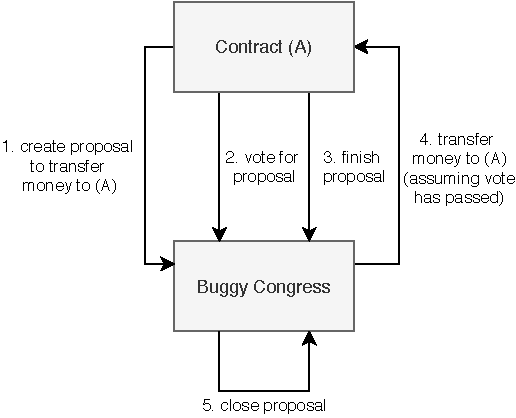
\includegraphics[width=0.65\textwidth]{media/congress-reentrancy.pdf}
\end{center}
\caption{Example scenario of the life-cycle of a proposal in the buggy Congress.}
\label{fig:buggy-congress-proposal}
\end{figure}
The last part is key, because what (A) then might do (not pictured in the diagram) is to call \finishproposal{} once more when it receives the money. If the underlying execution model executes actions \textit{depth-first}, then this new \finishproposal{} may be executed before step 5 when the buggy Congress closes the proposal. When it receives this message, it happily executes the transfer to (A) again. (A) can in principle continue to repeat this pattern until the buggy Congress contract runs out of money.
It is clear that the vulnerability stems from the fact that finishing a proposal is split into two steps, temporarily leaving a ``dangling'' invalid state until the proposal has been properly closed. The Congress contract avoids this vulnerability by closing the proposal before sending out the \congressAction{}s to be executed. Essentially, it swaps the order of step 4 and 5 in \autoref{fig:buggy-congress-proposal}.
We now want to state a testable property that guards against re-entrancy attacks on \finishproposal{}. As discussed in \cite{nielsen2019smart}, previous research which has focused on stating these types of properties often heavily rely on the benefit of hindsight, and the particular nature of the attack. This is hardly useful if we want to ensure that our contracts are safe against new, unknown attacks. In \cite{nielsen2019smart} they make the following observation: any transaction that is sent out by the Congress as a result of a successful, finished proposal should correspond to an action present in a previous \createproposal{} message. Formally, they state and prove (a simplification of) this property in Coq from the lemma, where \coq{num\_cacts\_in\_state} is a function that counts all \coq{Action}s in all active proposals.
\begin{code}
\label{def:cacts_preserved-receive_state_well_behaved}
\begin{minted}[escapeinside=\\$\\$]{coq}
  Definition proposal_cacts msg := 
    match msg with
    | Some (create_proposal ls) => length ls
    | _ => 0
    end.
  
  Definition cacts_preserved new_state resp_acts old_state msg :=
    num_cacts_in_state new_state + length resp_acts <=
    num_cacts_in_state old_state + proposal_cacts msg
    
  Lemma receive_state_well_behaved
      chain ctx state msg new_state resp_acts :
  receive chain ctx state msg = Some (new_state, resp_acts) ->
  cacts_preserved new_state resp_acts old_state msg.
\end{minted}
\end{code}
 Their proof of this lemma is about 150 lines in total. The lemma states that for any \coq{receive} step of the Congress, the number of actions in previous \createproposal{}s is always greater than or equal to the total number of actions the Congress has sent out. In particular, this safety property guards against the re-entrancy attack above. How can we make a testable representation of this property that we can test using our framework? We first notice that the property is stated over a single \coq{receive} step, so our pre-post condition checker is a natural fit. The post-condition we need to test is simply \coq{cacts\_preserved}. Note that this is a decidable proposition because $\le$ over natural numbers is decidable, so we can re-use this definition for our test property since decidable propositions are testable, as we discussed in \autoref{sec:obt-qc}. We easily prove this decidability, as shown below. For readers unfamiliar with Coq proofs, the proof below essentially just unfolds definitions and applies an existing proof, \coq{le\_dec} that shows $\le$ is decidable for natural numbers.
\begin{code}
\label{def:receive_state_well_behaved_dec}
\begin{minted}[escapeinside=\\$\\$]{coq}
  Lemma receive_state_well_behaved_dec :
    forall state msg new_state resp_acts,
      Dec (receive_state_well_behaved state msg new_state resp_acts).
    Proof.
    intros. unfold receive_state_well_behaved. 
    constructor. 
    apply le_dec.
    Qed.
\end{minted}
\end{code}
With this, we can easily define the post-condition property, and test whether Buggy Congress satisfies this property.
\begin{code}
\label{def:receive_state_well_behaved_P}
\begin{minted}[escapeinside=\\$\\$]{coq}
  Definition receive_state_well_behaved_P 
    (cctx : ContractCallContext) 
    (old_state : Congress.State) 
    (msg : Congress.Msg) 
    (result : option (Congress.State * list ActionBody)) := 
  match result with
  | Some (new_state, resp_acts) =>
    (receive_state_well_behaved old_state (Some msg) new_state resp_acts)?
  | _ => false
  end.

  QuickChick (
    {{fun _ _ => true}}
    Congress_Buggy.contract
    {{receive_state_well_behaved_P}}
  ).
\end{minted}
\end{code}
However, QuickChick reports that all tests passed. Why? Because the re-entrancy attack relies on some deployed, malicious contract, but the chain we tested on only had the Congress contract deployed on it. If we deploy a malicious contract such as the one described before, which just repeatedly calls \finishproposal{} when it receives any incoming transaction, QuickChick now fails with a counterexample:
\begin{code}
\begin{minted}[escapeinside=\\$\\$]{coq}
  Begin Trace: 
    step_action{Action{
      act_from: 10, 
      act_body: (act_call 128, 0, create_proposal (transfer: 10, 1))}};;
    step_action{Action{
      act_from: 10, 
      act_body: (act_call 128, 0, finish_proposal 1)}}
  End Trace
\end{minted}
\end{code}
In this trace the address \coq{128} refers to the malicious contract. Indeed, the execution trace we see is similar to the one described earlier. The malicious contract is coded to perform 25 re-entrancy attacks. If we inspect the balance of the account with address \coq{10} after the last step, it will have increased by 25 (assuming the buggy Congress had at least this much money), since the proposed transfer was with an amount of 1. If we execute the same test on the (non-buggy) Congress contract, it will of course find no counterexamples.

\subsection{Summary}
In this case study we presented the Congress contract, a simplified version of the DAO designed to be safe against the re-entrancy attack on the DAO which resulted in a loss of \$50 million worth of cryptocurrency. We tested a black-box safety property guarding against this re-entrancy attack on a buggy implementation of the Congress contract which has the same vulnerability as the DAO. Our testing framework was able to discover an execution trace violating this property, only requiring a simple adversarial contract to be deployed on the blockchain along with the buggy Congress. 
We also showed how our testing approach also supports sharing parts of the properties between testing and verification efforts. This is a concrete example of how testing and verification and be combined; suppose we had not yet proved \coq{receive\_state\_well\_behaved}, but wished to do so. We could first have tested it. For the buggy Congress, our testing framework would have discovered a counterexample violating the property if only we had deployed a generic, malicious re-entrancy contract in our test blockchain. In the non-buggy Congress it would find no such counterexamples, so we could proceed to formally prove the property, now with more certainty that our proving efforts will be successful.

\section{FA2 Tokens}
\label{sec:fa2}
FA2 is a proposal for a multi-asset interface designed to support various types of tokens on the Tezos blockchain\cite{tzip12-fa2}. It was first publicized on the 21st of January in 2020, and is at the time of writing still an early-stage draft and until the 6th of May 2020, no complete reference implementation existed\cite{fa2-python}. Hence, the specification is a key target for testing. In this case study we present the specification of the FA2 and describe our implementation as a ConCert smart contract. We then proceed to test some properties stated in the specification. In \autoref{sec:uniswap} we combine our FA2 contract with a liquidity contract to test a recently discovered vulnerability.

\subsection{The FA2 Interface}
\label{sec:fa2-interface}
Tokens play an important role on blockchains since they can be used to represent real-world assets. There are many token interfaces, such as ERC-20, ERC-777, ERC115, each with their own unique properties. For example, tokens are usually categorized by whether they are \textit{fungible} or \textit{non-fungible}. Fungible tokens of the same type represent non-unique, comparable assets like real-world money, and may be convertible to other fungible tokens. On the other hand, non-fungible tokens represent unique, non-interchangeable assets like certificates or identifications. The current landscape of token standards is very fragmented, and most existing token standards support only one of these token types. The FA2 interface is designed to support various token types, and to provide developers with a wide latitude of options to define and invent their own token types with their own, complex interactions, while maintaining a standard API for external applications. The goal of the FA2 interface is to provide a common standard for most use-cases of tokens\footnote{Although a common standard may never be realistically possible; cf. \url{https://xkcd.com/927/}}, and to standardize handling of token permissions.\medskip\\
A token contract implementing the FA2 standard must have the following endpoints, as defined in cameLIGO notation:
\begin{itemize}
    \item \coq{Transfer of transfer list}
    \item \coq{Balance\_of of balance\_of\_param}
    \item \coq{Total\_supply of total\_supply\_param}
    \item \coq{Token\_metadata of token\_metadata\_param}
    \item \coq{Permissions\_descriptor of permissions\_descriptor contract}
    \item \coq{Update\_operators of update\_operator list}
    \item \coq{Is\_operator of is\_operator\_param}
\end{itemize}
The complete list of related type declarations can be found in \autoref{ch:appendix-fa2-interface-types}. We encourage the reader to revisit this appendix whenever needed. We will focus on describing the \coq{Transfer} and \coq{Update\_operators} endpoints, and refer to the official specification for the full description\cite{tzip12-fa2}. An FA2 token contract applies permission policy logic through its current \coq{permissions\_descriptor}, which is defined as
\begin{minted}{ocaml}
  type permissions_descriptor = {
    self : self_transfer_policy;
    operator : operator_transfer_policy;
    receiver : owner_transfer_policy;
    sender : owner_transfer_policy;
    custom : custom_permission_policy option;
  }
\end{minted}
The permission descriptor specifies whether self transfers and operator transfers are allowed, and if so, on which token ids they are allowed. It can also support custom \textit{transfer hooks} to the sender/receiver, which will approve or reject the transaction. These hooks may also be used for purposes beyond permissions, for example by implementing custom logic as a consequence of a failed or successful transaction. It may also implement an optional, custom permission policy in a separate contract in the \coq{custom} field.
The \coq{Transfer} endpoint is a batch operation where each \coq{transfer} operation is defined as:
\begin{minted}{ocaml}
  type token_id = nat
  type transfer = {
    from_ : address;
    to_ : address;
    token_id : token_id;
    amount : nat;
  }
\end{minted}
The specification states that transfers must happen atomically, i.e. if at least one transfer fails then the entire operation should fail. The transfer must apply permission policy logic, as defined by the current \coq{permissions\_descriptor}. Transfers must update the balances only as specified in the \coq{transfer}s. In particular, they may not add additional transaction fees.

In FA2 an operator is an address that initiates a token transfer on behalf of the owner. This is similar to the \coq{approve}/\coq{transfer\_from} behavior of the ERC-20 specification. The definitions related to \coq{Update\_operators} are shown below
The \coq{Transfer} endpoint is a batch operation, where \coq{transfer} is defined as:
\begin{minted}{ocaml}
  type operator_tokens =
  | All_tokens
  | Some_tokens of token_id set
  type operator_param = {
    owner : address;
    operator : address;
    tokens : operator_tokens;
  }
  type update_operator =
  | Add_operator of operator_param
  | Remove_operator of operator_param
\end{minted}
The \coq{Update\_operators} entry point accepts a list of \coq{update\_operator}s. The specification states that if two different operations add and remove the same operator for the same owner and token type, then the \textit{last} occurring operation must take effect. Note that if an operator is allowed to operate on \coq{All\_tokens}, then if some new token type is added later on, it will also be allowed to operate on this token type. Only operators are allowed to transfer tokens on behalf of other token holders, and only if the permission policy allows operator transfers.

\subsection{Implementation in ConCert}
\label{sec:fa2-implementation}
Several of the FA2 endpoints are endpoints that do not modify the state of the contract, and only ``return'' some information about the state. Namely the endpoints
\begin{itemize}
    \item \coq{Balance\_of of balance\_of\_param}
    \item \coq{Total\_supply of total\_supply\_param}
    \item \coq{Token\_metadata of token\_metadata\_param}
    \item \coq{Permissions\_descriptor of permissions\_descriptor contract}
    \item \coq{Is\_operator of is\_operator\_param}
\end{itemize}
But the concept of ``returning'' data does not immediately fit ConCert's execution model. In ConCert, contracts can only send and receive \coq{Action}s using a message-passing paradigm. We can implement the concept of returning data with callbacks, as illustrated in \autoref{fig:callback-ex} for the \coq{Balance\_of} endpoint. 
\begin{figure}[h]
\begin{center}
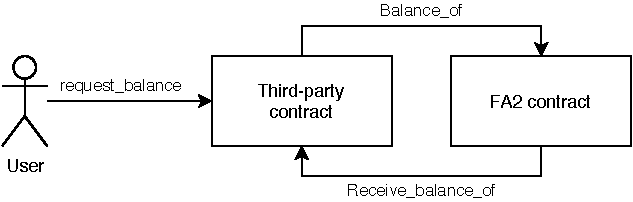
\includegraphics[width=0.7\textwidth]{media/balance_of_callback.pdf}
\end{center}
\caption{Example implementation of the life-cycle of the \coq{Balance\_of} endpoint.}
\label{fig:callback-ex}
\end{figure}
This requires that the \coq{Msg} type of has some constructor named \coq{Receive\_balance\_of} in this example. In our implementation, we generalize this and require that any third-party contract of the FA2 contract should be able to receive any of the callback endpoints listed above. We ensure this by requiring that these contracts receive messages of the \coq{FA2ReceiverMsg} type:
\begin{code}
\begin{minted}[escapeinside=\\$\\$]{coq}
  Inductive FA2ReceiverMsg {Msg' : Type} `{Serializable Msg'} :=
  | receive_balance_of_param : list balance_of_response -> FA2ReceiverMsg
  | receive_total_supply_param : list total_supply_response -> FA2ReceiverMsg
  | receive_metadata_callback : list token_metadata -> FA2ReceiverMsg
  | receive_is_operator : is_operator_response  -> FA2ReceiverMsg
  | receive_permissions_descriptor : permissions_descriptor -> FA2ReceiverMsg
  | other_msg : Msg' -> FA2ReceiverMsg.
\end{minted}
\end{code}
Note that the \coq{other\_msg} constructor allows the contract to have other endpoints than these. In particular, it allows the scenario in \autoref{fig:callback-ex} if \coq{Msg'} contains a \coq{request\_balance} constructor. In a way we can view this as method for \textit{composing} contract endpoints in ConCert. When one of the callback endpoints of the FA2 contract is called, it will return a \coq{act\_call} action with a \coq{FA2ReceiverMsg} message.

The FA2 Specification recommends a transfer hook pattern, as discussed earlier. This enables separation of the core token transfer logic and the permission policy logic. It also makes it possible to have different transfer logic for different token types. Another benefit is that the core FA2 implementation can be verified in isolation from custom external transfer logic. In our implementation, we support transfer hooks in the following way: the FA2 contract has an optional transfer hook address. When the contract receives an incoming transfer, if the transfer hook is set, it will immediately forward the transfer to the hook and wait for its response before it carries out the transfer. If the hook it not set, it will immediately carry out the transfer. It only applies the permission policy to the transfers if the hook is set, since the idea is that the hook should be responsible of permission policy. \autoref{fig:transfer-hook} illustrates the scenario where the transfer hook is set.
\begin{figure}[h]
\begin{center}
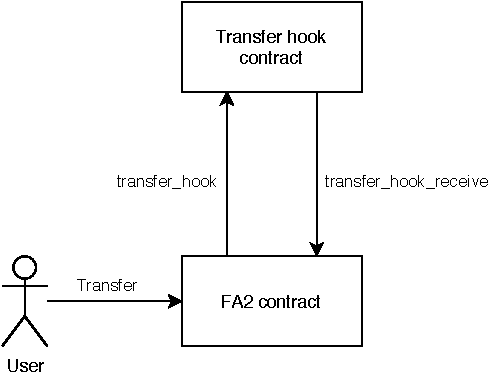
\includegraphics[width=0.55\textwidth]{media/fa2_transfer_hook.pdf}
\end{center}
\caption{Transfer life-cycle using external transfer hook contract.}
\label{fig:transfer-hook}
\end{figure}
In our implementation the transfer hook contract is trusted by the FA2 contract to not behave adversarially. In particular, we assume that if it accepts a transfer by sending the transfers back to the FA2 contract, it will not have modified, added, or removed any of the transfers. We chose this approach to simplify the implementation. A production-ready implementation should choose a different approach requiring less trust in the hook transfer contract. The core logic of our implementation is about 400 lines of Coq code. We omit further implementation details and refer the interested reader to the source code\footnote{Our FA2 implementation is available \href{https://github.com/mikkelmilo/ConCert/blob/master/execution/theories/Examples/FA2Token.v}{here}.}

\subsection{Testing the Implementation}
In this section we discuss how to test our implementation against the specifications of \coq{Transfer} and \coq{Update\_operators}, as presented in \autoref{sec:fa2-interface}. Like in the other case-studies, we first need to implement a generator of FA2 actions. This generator follows a similar implementation methodology as the generators presented in the other case studies, and does not provide much new insight, so we omit the implementation here. Hence, we can assume in the following that we have some trace generator where the generated actions to be executed in each block contain arbitrary FA2 messages. We refer the interested reader to the source code\footnote{The FA2 Generator implementation is available \href{https://github.com/mikkelmilo/ConCert/blob/master/execution/tests/FA2Tests/FA2Gens.v}{here}}.


First we consider how to state that \coq{Transfer} updates the balances correctly. Since the \coq{Transfer} endpoint accepts a list of transfers to be executed as a batch operation, we need to state the property as the balance changes before and after \textit{all} transfer operations have been performed. We can easily compute a mapping \coq{FMap Address nat} that records the difference in balance for each token owner after some batch operations of transfers has been executed. Given the previous and new state of the FA2 contract, we can then compare if the balances has been updated according to this mapping. Suppose \coq{transfer\_state\_update\_correct} is a function asserting this specification. As usual, we could then state and test the specification on \coq{Transfer} as a one-step, functional property on the \coq{receive} function of the FA2 contract:
\begin{code}
\begin{minted}[escapeinside=\\$\\$]{coq}
{{ msg_is_transfer }} 
  FA2Token.contract 
{{ transfer_state_update_correct }}
\end{minted}
\end{code}
If we execute this test on a chain where the FA2 contract has been configured to \textit{not} use a transfer hook (meaning it will execute transfers immediately when it receives them), then QuickChick will report that all tests passed. However, if we test it on a chain where the FA2 contract uses a transfer hook contract, then it immediately fails, even if the transfer hook contract never rejects any transfer. Why? Because the life-cycle of the transfer now spans across multiple contract calls. Thus, we cannot properly state the specification using the pre-post condition checker above. However, the entire life-cycle of the transfer still occurs within the same block. Therefore, we can instead use the \coq{forAllTraces} checker, which tests properties over steps (recall that one step is exactly one block). This illustrates how we can test ``step'' properties at different granularity with the checkers available in our testing framework. 

The specification states that transfers must be consistent with the current permission policy. Namely, if the permission policy is configured to disallow operator transfer, then any transfer initiated by an operator must fail. Similarly, if the permission policy disallows owner transfers, then any transfer initiated by the owner must fail. We test that our permission policy logic implements this behavior with a similar approach as before with the \coq{forAllTraces} checker, and a suitable Coq definition that asserts any transfer is consistent with the current permission policy. QuickChick passes all tests on these properties, which gives us confidence that our implementation is correct.  

As described in \autoref{sec:fa2-interface}, the \coq{Update\_operators} endpoints must update operators in such a way that if there are two updates on the same operators, the last one should be applied. It is not too hard to imagine how one could implement a function that checks this property. It should just discard all the updates which should not be executed, and check that only those \coq{update\_operator} operations have been executed. We omit the actual Coq definition since it provides no useful insight. For reference, our Coq definition of this property is about 30 lines. We use this property as the post-condition of a single \coq{receive} step of the FA2 token, and test it in the usual way:
\begin{code}
\begin{minted}[escapeinside=\\$\\$]{coq}
QuickChick (
  {{msg_is_update_operator}}
  FA2Token.contract
  {{last_update_operator_occurrence_takes_effect}}
).
\end{minted}
\end{code}
QuickChick finds no counterexample, and passes all (10.000) tests (with 65.772 discards).
\subsection{Summary}
In this case study we presented the FA2 token standard, and our implementation in ConCert. We tested our implementation against the specification for the \coq{Transfer} and \coq{Update\_operators} endpoints with positive results. QuickChick found no counterexamples during testing, so we are fairly confident that our implementation indeed satisfies the specification. In the next case study we use our FA2 contract in conjunction with a liquidity contract, Dexter, to test for a recently discovered vulnerability of the UniSwap protocol.

\section{The UniSwap Exchange Re-entrancy Exploit}
\label{sec:uniswap}
A recent, successful attack on the \href{https://uniswap.org/}{Uniswap} liquidity protocol was conducted by exploiting a re-entrancy vulnerability that is present in \textbf{any Uniswap exchange that uses ERC777 compliant tokens}. The purpose of this section is to study the attack and to see if we can use our testing framework to state and test a safety property guarding against this kind of re-entrancy attack.

\subsection{Uniswap Vulnerability with ERC777 Tokens}
\label{sec:uniswap-intro}
Uniswap is a publicly available, open-source protocol to support exchanges of assets such as fungible tokens on the Ethereum blockchain. It was originally designed to support any compliant ERC-20 tokens by having a separate exchange contract for each token type. Tokens can be exchanged for Ether (the currency of the Ethereum blockchain), and vice versa. The exchange rate depends on the current reserves of Ether and tokens held by some central, liquidity-providing contract. A successful exchange from tokens to ether is executed in the following steps:
\begin{enumerate}
    \item calculate the exact exchange rate
    \item send corresponding Ether to the caller
    \item transfer tokens to the liquidity contract
\end{enumerate}
The exchange rate is calculated according to the formula
\begin{equation*}
\begin{split}
getInputPrice &= \frac{Ts \cdot 997 \cdot ETHr}{Tr \cdot 1000 + Ts \cdot 997}\\
\text{where}&\\
Ts&: \text{nr. of tokens being sold by caller} \\
Tr&: \text{current token reserve held by the liquidity contract} \\
ETHr&: \text{current Ether reserve held by the liquidity contract}
\end{split}
\end{equation*}
The exchange rate influences the prices in the following way: after a sale of tokens, the current reserve of tokens ($Tr$) increases, so the denominator increases. Similarly, since the current reserve of Ether ($ETHr$) decreases, then the numerator also decreases. In effect, the price of tokens decreases when tokens are sold, and vice versa when tokens are bought.

We now describe how to exploit the Uniswap protocol to exchange tokens at unintended exchange rates to obtain an unintended profit in Ether. This exploit is possible if the tokens we exchange are ERC-777 tokens, which is an ERC-20 compliant token implementation. The only detail we need to know about ERC-777 tokens is that they have transfer hooks. In any transfer of an ERC-777 token, the following happens in this exact order:
\begin{itemize}
    \item A call is made to the \textit{sender}, notifying them of the transfer that is about to occur
    \item the token transfer is executed (i.e. token balances are updated correspondingly)
    \item A call is made to  the \textit{recipient}, notifying them of the transfer that has just occurred 
\end{itemize}
Note that senders and recipients can be contracts. This means that the sender can \textbf{execute arbitrary code \textit{before} the transfer occurs}. This is problematic because when the sender is called, the Uniswap/liquidity contract is in a state where the Ether reserves have already been reduced, and Ether has been sent to the sender, but the token reserve has not yet been reduced. If the sender is a contract, they can perform a re-entrancy on the token exchange operation. Since $Tr$ has not yet been reduced, the price of tokens becomes cheaper than expected, and so the attacker will have made a profit in this second token exchange. In \autoref{fig:microtrading-example} we illustrate a concrete example where an attacker is able to obtain a profit of 33\% from selling 1000 tokens compared to legitimate exchanges selling the same amount of tokens.
\begin{table}[h]
\centering
\begin{tabular}{ |c|c|c|c|c| } 
\hline
Scenario & Description & Tokens sold & ETH received \\
\hline
\multirow{2}{6em}{Legitimate exchange (1)} & \multirow{2}{10em}{A user exchanges 1000 tokens}&1000& \textasciitilde 12 \\
&&&\\
\hline
\multirow{2}{6em}{Legitimate exchange (2)} & \multirow{2}{10em}{A user exchanges 200 tokens 5 times} &1000& \textasciitilde 12 \\
&&&\\
\hline
\multirow{2}{6em}{Exploiting exchange}  & \multirow{4}{10em}{An attacker (contract) initiates a transfer of 200 tokens, an then performs 4 re-entrant exchanges, each of 200 tokens} &  1000 & \textasciitilde 16 \\
&&&\\
&&&\\
&&&\\
&&&\\
\hline
\end{tabular}
\caption{An example of how an attacker can obtain a profit by exploiting the re-entrancy vulnerability when using a token with transfer hooks in the Uniswap exchange protocol}
\label{fig:microtrading-example}
\end{table}
The attack is made possible due to the underlying execution model of smart contracts on Ethereum. It uses depth-first execution. This means if a contract $A$ sends out a queue $T_1,\dots,T_n$ of transactions to other contracts, when $T_1$ is received by some other contract $B$, any transactions sent out by $B$ will be executed \textit{before} $T_2,\dots T_n$ are executed. This is what allows an attacking contract to ``insert'' some transactions in the middle of some existing queue of calls to be executed. Depth-first execution essentially models a LIFO queue (i.e. a stack), whereas breadth-first execution models a FIFO queue. In the latter case the attack is not possible since the re-entrant exchanges are inserted at the bottom of the queue, so they will be executed after the token balances have been updated. In particular, as discussed in \cite{erc777-attacks-tezos}, this vulnerability does not exist on the Tezos blockchain since it uses breadth-first execution. The blockchain implementation we use in ConCert can be configured to use either execution model.

\subsection{Replicating \& Testing the scenario in ConCert}
How can we replicate the scenario in ConCert? We need a token contract with transfer hooks and a liquidity contract supporting exchange from tokens to money using the same exchange conversion formula as presented earlier. Recall that the FA2 token contract presented in \autoref{sec:fa2} supports transfer hooks, so we can use this contract for token transfers. For the liquidity contract, we use inspiration from the \href{https://gitlab.com/camlcase-dev/dexter/-/blob/master/dexter-contracts-ligo/dexter.ligo}{Dexter} token exchange contract on Tezos. Our Dexter-like contract exposes two endpoints:
\begin{code}
\begin{minted}[escapeinside=\\$\\$]{coq}
  Inductive DexterMsg :=
  | add_to_tokens_reserve : token_id -> DexterMsg.
  | tokens_to_asset : exchange_param -> DexterMsg
  
  Record exchange_param := {
    exchange_owner    : Address;
    exchange_token_id : token_id;
    tokens_sold       : N;
    callback_addr     : Address;
  }.
\end{minted}
\end{code}
The \coq{add\_to\_tokens\_reserve} may only be called by the owner of the contract. It adds FA2 tokens to the reserve of the Dexter contract. This reserve corresponds to $Tr$ in $getInputPrice$. \autoref{fig:dexter-exchange} shows the life-cycle of the \coq{tokens\_to\_asset} endpoint. When it is called, the Dexter contract will first calculate the price of the tokens to exchange according to the definition of $getInputPrice$, and then send out a monetary transaction to the caller. Then it sends out the token transfer to the FA2 contract with \coq{callback\_addr} as the callback address (usually the initiating address of the token exchange). The description we provided is a simplified version of the actual behavior. Here we have assumed that if the caller is a contract wanting to transfer tokens on behalf of some user, then it has already been added as an operator for this user on the FA2 contract. We have also assumed that the token owner has enough tokens to exchange, and that on deploy, the Dexter contract is given sufficient money to perform this token exchange.
\begin{figure}[h]
\begin{center}
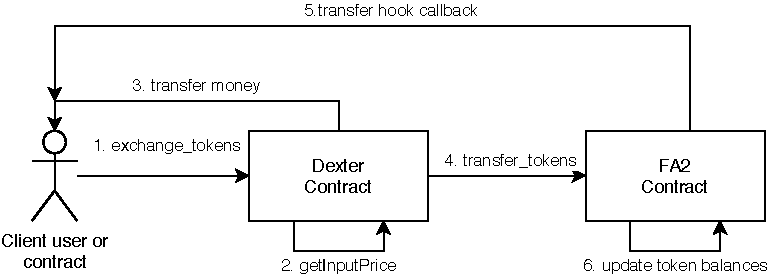
\includegraphics[width=0.95\textwidth]{media/Dexter-exchange-diagram.pdf}
\end{center}
\caption{Token exchange life-cycle in our Dexter+FA2 set-up}
\label{fig:dexter-exchange}
\end{figure}
With the liquidity/token exchange set-up completed, we turn our attention to the attacking contract. Luckily, this is a very simple contract with nearly identical behavior to the attacking contract of the DAO/buggy Congress attack from \autoref{sec:congress-example}. The exploit contract has a single endpoint which also acts as the transfer hook callback as shown in step 5 in \autoref{fig:dexter-exchange}. When this endpoint is called, it initiates another call to the \coq{tokens\_to\_asset} endpoint of the Dexter contract, causing the re-entrancy. To make testing easier, we have specialized the attacking contract to repeat re-entrancy up to five times with the same transfer of 200 tokens on behalf of the same user. In our set-up of the blockchain we make sure to add the exploit contract as an operator on behalf of this user, and transfer some tokens to the user so they can actually perform the exchange.

We now consider how to state a safety property the guards against such a re-entrancy attack. We want the property to be defined independently of attack. In other words, the property should be one we could conceive without prior knowledge of the attack. We state the safety property based on an observation on $getInputPrice$ in the two legitimate token exchange scenarios in \autoref{fig:microtrading-example}. Under normal operation, $getInputPrice$ should satisfy the following property. Given two arbitrary sequences, $s_1$ and $s_2$, of token exchanges from the same user on the same token type. Let $n_1$ ($n_2$) be the total number of tokens exchanged in $s_1$ ($s_2$), and let $m_1$ ($m_2$) be the total amount of money received after all exchanges in $s_1$ ($s_2$) have been executed successfully from the same initial state (assuming no other exchanges/transfers have occurred in in between). If $n_1 = n_2$ then $m_1 = m_2$. Intuitively, what this property says is that it does not matter if we transfer 1000 tokens in one exchange, or 1000 tokens spread out in several exchanges (as long as no other exchanges or transfers occur in between). The legitimate exchanges described in \autoref{fig:microtrading-example} are an example of this property. They both transfer 1000 tokens in total, and they both receive the same amount of Ether. Note that this property does not mention any kind of attack or vulnerability. It is purely a safety/correctness property on $getInputPrice$. We can state this as a testable property in Coq, \coq{tokens\_to\_asset\_correct\_P}, by computing an \textit{expected} token and monetary balance (using $getInputPrice$) of the Dexter contract, and compare it with its \textit{actual} balances. We assert this property on any step of an execution trace, and test it with
\begin{code}
\begin{minted}[escapeinside=\\$\\$]{coq}
  QuickChick (forAllExploitExTraces tokens_to_asset_correct_P).
\end{minted}
\end{code}
where \coq{forAllExploitExTraces} is the \coq{forAllTraces} checker specialized to the chain set-up we described earlier. QuickChick immediately reports a counterexample where the exploit contract has exchanged 200 tokens five times in a row, The Dexter contract has transferred 16 tokens in total to the owner, but the expected number was 12, just like in the example in \autoref{fig:microtrading-example}.

\subsection{Summary}
In this small case-study of the recently discovered vulnerability in UniSwap we tested the vulnerability on a similar set-up in ConCert. We found that the vulnerability only exists whenever the execution model is depth-first. The safety property we defined to guard against this vulnerability was defined completely independent of the actual attack, illustrating how we can state safety properties for re-entrancy that does not depend on the benefit of hindsight of the concrete attack vector.

%%%%%%%%%%%%%%%%%%%%%%%%%%%%%%%%%%%%%%%%%%%%%%%%%%%%%%%%%%%%%%%%%%%%%%%

\chapter{Discussion}
\label{ch:evaluation}
In this chapter we briefly discuss and evaluate whether we have satisfied the goals stated in \autoref{ch:intro}, based on our findings of the case studies in \autoref{ch:case-studies}. Many key discussion points have already been addressed in earlier chapters, in particular in the case studies, and we do not intend to reiterate them all here.
\medskip\\
The approach we have taken to support \pbt{} on smart contracts is based on generating valid execution traces and defining \textit{checkers} over these execution traces that test some specific type of property like reachability or functional properties.
\medskip\\
\textbf{Quality of test data.} Our first concern is to which degree our approach supports high quality test data, since this be a prerequisite for high quality, useful tests. As discussed in \autoref{sec:obt-qc} the quality of test data can be measured with respect to how \textit{realistic} it is, and whether there is a sufficient degree of \textit{variation} in the test data. Otherwise the tests will not be able to cover a large part of the input scope of the function under test. The generator approach taken by QuickChick sacrifices some automation in order to provide better tools for the programmer to state custom, high quality input generators. This can both be a advantage and a disadvantage, since the quality of the input generators depends on the skill of the developer. An inexperienced developer might not be able to implement generators of sufficient quality to discover bugs during testing. This applies to our testing framework as well, since the generators for actions/contract calls of the contracts under test must be supplied by the user. However, with the tooling provided by both QuickChick and our testing framework, we believe that users are well-equipped to implement generators of sufficiently high quality. Determining whether the generators have sufficient quality is related to how well they can discover bugs.
\medskip\\
\textbf{Finding bugs with \pbt{}.} The primary purpose of testing is to find bugs. The degree to which a \pbt{} library such as QuickChick can find bugs depends on the quality of the input generators, and the way the properties to test are stated. In our case studies we have shown that our testing framework supports complex properties, and is capable of discovering known, crucial vulnerabilities in contracts. Even when the stated safety property relies on no knowledge of the concrete attack. A small caveat on finding re-entrancy bugs is that we must manually implement and deploy an attacking contract on the test chain, which does imply some a priori knowledge of the attacks we wish to guard against. Thus, our approach to testing re-entrancy attacks is not entirely opaque to the concrete attack vectors, which is a disadvantage of our approach. 
\medskip\\
\textbf{Supporting testing of complex contract interactions.} Existing \pbt{} libraries for smart contracts all share the same characteristic that they only support testing of contracts in isolation. However, as illustrated by the UniSwap vulnerability, sometimes the vulnerability does not lie in a single contract, but in the interactions between multiple contracts. Our testing framework supports stating and testing properties on entire execution traces, which is what allows us to state properties of contract interactions. We have demonstrated this in practice in both our re-entrancy tests and our test of the UniSwap vulnerability, where our testing framework successfully discovered the execution traces of interacting contract calls that violated the stated safety properties. Existing testing libraries would not be able to discover these vulnerabilities. Our experience with the testing framework shows that stating complex, testable properties can sometimes be more difficult than when stating propositions for verification. This is because testing requires that the property is \textit{executable}. 
\medskip\\
\textbf{Testing of contracts in conjunction with formal verification.}
Our testing framework is developed in the Coq proof assistant for the \cc{} blockchain formalisation and smart contract execution framework. Having both formal proofs and test on the exact same code base is of course an advantage in itself. QuickChick further supports combining testing and verification efforts by providing automation with some typeclasses (\coq{Dec} and \coq{Dec\_Eq}) that allow, to some extent, to test on the same propositions as one might prove as long as the propositions are \textit{decidable}. We utilize this in our testing framework, and as demonstrated in our case study of the Congress, we were able to re-use central parts of a proposition that was proved in \cite{nielsen2019smart} that asserts the Congress is not vulnerable to re-entrancy attacks. Some properties cannot be shared between testing and verification. For example, universal and existential quantification can of course not be tested in a way where the test result is both sound and complete. In these cases we must make approximations when testing.

\chapter{Conclusions}
\label{ch:conclusion}
We have developed a \pbt{} framework for ConCert, a blockchain formalisation in Coq, using QuickChick. Our approach is based on automatically generating arbitrary, valid execution traces for testing from semi-automatically derived generators. 
This means we can define testable properties over \textit{entire} execution traces, unlike existing \pbt{} frameworks for smart contracts, which only allow testing single steps of execution. In particular, our approach allows us to state and test both functional and temporal properties describing complex contract interactions. We have demonstrated these capabilities of our framework in various case studies such as ERC-20 tokens, the Congress, FA2 tokens, and the UniSwap token exchange platform, where we implemented these contracts in ConCert, and tested key properties on them. We used our testing framework to successfully discover well-known vulnerabilities such as a vulnerability in transfers of ERC-20 compliant tokens, the re-entrancy vulnerability on the DAO, and a recently discovered re-entrancy vulnerability in the UniSwap protocol. We found these vulnerabilities using our testing framework by stating safety properties, either as functional of temporal properties. 

Thus, we have shown not only the feasibility of using \pbt{} on smart contracts, but also its effectiveness. We have also demonstrated how testing and verification efforts can be combined. In part, this is due to the fact that both ConCert and our testing framework are developed in the Coq proof assistant, but also because QuickChick allows, to some extent, testing on the same specification that one intends to prove. This means testing can be used as a preliminary, cost-effective step in the process of formal verifying a (collection of interacting) contract(s) in order to potentially discover bugs. We demonstrated this in our tests of the Congress contract.


\chapter{Future Work}
\label{ch:future-work}
\textbf{Improved automation.} Our testing framework relies on deriving execution trace generators. These are typically composed from custom implemented generators for endpoints of the contracts we test. Currently, these have to be implemented manually, and while we do provide tools for making this process easier, it can still require significant work. QuickChick supports automatically deriving generators of inductive propositions. This may be used to support a different approach to implementing input generators for contracts by stating the properties their endpoints should satisfy as inductive propositions, and then automatically derive generators satisfying these propositions. Currently QuickChick only supports very restricted inductive propositions, so in more complex contracts it may not be possible yet. In \cite{lampropoulos2016beginners} they develop Luck, a domain-specific language for deriving generators satisfying predicates, and they prove soundness of their development. This could be used in a similar way to simplify and partially automate derivation of trace generators.
\medskip\\
\textbf{Certified input generators.} The input generators and combinators we define and use in our testing framework are not formally verified. In other words, we have no guarantee that the data they generate is valid. As discussed previously, this is usually not an issue since, intuitively, the way we generate traces (intuitively) ensure that they are valid. However, if we want to improve integration with verification efforts, it is beneficial to have certified input generators. Of course, this also increases trust of the testing framework in general. QuickChick supports certifying generators by proving that the elements they generate belong to some set.
\medskip\\
\textbf{Shrinking for minimal counter examples.} In \autoref{ch:quickchick} we briefly mentioned \textit{shrinkers} which somehow ``shrink'' counterexamples. This makes it easier for the user to detect exactly which part of the counter example violated the test case. We have not used shrinkers in our testing framework, but they could be beneficial when testing blockchain execution traces because generated execution traces may be very long and contain many irrelevant actions for the particular test case. Shrinking of execution traces is not trivial though, since the shrunk trace must also be a valid execution trace. For example, in the EIP-20 token contract, a relevant \coq{approve} action must occur before a \coq{transfer\_from}. Suppose a shrinker shrinks an execution trace by removing some actions executed in the blocks. Then it might remove an \coq{approve} message, but this could cause the execution trace to become invalid if there were any relevant \coq{transfer\_from} actions in succeeding blocks. This also motivates certification of the generators and shrinkers.

%%%%%%%%%%%%%%%%%%%%%%%%%%%%%%%%%%%%%%%%%%%%%%%%%%%%%%%%%%%%%%%%%%%%%%%

\cleardoublepage
\addcontentsline{toc}{chapter}{Bibliography}
\bibliographystyle{plain} 
\bibliography{bibliography}

%%%%%%%%%%%%%%%%%%%%%%%%%%%%%%%%%%%%%%%%%%%%%%%%%%%%%%%%%%%%%%%%%%%%%%%

\cleardoublepage
\appendix


\chapter{QuickChick Example: Testing Confluence of Lambda Calculus}
\label{ch:appendix-qc-example}
This chapter aims to provide an simple yet interesting example of how to use QuickChick for testing. The purpose is to apply the features of QuickChick described in \autoref{sec:obt-qc} on a concrete, illustrative example.

The most common examples used to present QuickChick and similar \pbt{} frameworks are based on testing properties of lists or binary trees. While these examples are indeed illustrative, they are not very interesting due to their overuse. Instead we choose a novel example that, in the authors' opinion, is significantly more interesting and motivating.

The untyped lambda calculus is a well-studied formal system used either as a universal model of computation, as a core for functional programming languages or, by the Curry-Howard Isomorphism, even as a formal theory in field of proof theory. Many formalisations of the lambda calculus in proof assistants have been made \cite{koprowskiformalization}\cite{swords2006soundness}\cite{segundoformalizing}\cite{aydemir2007nominal}. The main concern is usually to prove that with $\beta$-reduction (or other reduction schemes), the lambda calculus becomes a \textit{confluent} rewriting system, also referred to as the \textit{Church-Rosser} property, or sometimes informally called the \textit{diamond} property. The goal of this example is test (a corollary of) confluence/Church-Rosser on the lambda calculus using QuickChick. The scenario or use-case we imagine here is that we wish to develop (yet another) formalisation of the lambda calculus with the ultimate goal of proving confluence. Since we know this property holds for the lambda calculus with $\beta$-reduction, we expect to be able to prove this property, however if we have made any implementation errors along the way, this could cost us significant wasted time and efforts in trying to prove a property that does not hold. To avoid this we first test the property to potentially discover any coding mistakes. This is the scenario we imagine. The Coq definitions we use for lambda terms and $\beta$-reduction are inspired by \href{https://github.com/pi8027/lambda-calculus}{this formalisation in Coq}. The most central definitions are shown below
\begin{code}
\begin{minted}[escapeinside=\\$\\$]{coq}
(* de-brujin style untyped lambda terms *)
Inductive term : Set := 
  | var of nat 
  | app of term & term 
  | abs of term.

(* decision procedure for equality on lambda terms *)
Fixpoint eqterm t1 t2 :=
  match t1, t2 with
    | var n, var m => n == m
    | app t1l t1r, app t2l t2r => eqterm t1l t2l && eqterm t1r t2r
    | abs t1, abs t2 => eqterm t1 t2
    | _, _ => false
  end.

(* use eqterm for equality (=) on terms. Proof not shown. *)
Lemma eqtermP : Equality.axiom eqterm.
Proof. ... Qed.

(* computing beta normal form of a term *)
Definition reduce_all_redex t : term :=
  match t with
    | var _ => t
    | app (abs t1) t2 =>
      substitute 0 [:: reduce_all_redex t2] (reduce_all_redex t1)
    | app t1 t2 => app (reduce_all_redex t1) (reduce_all_redex t2)
    | abs t' => abs (reduce_all_redex t')
  end.

(* A relational definition of beta reduction *)
Inductive betared : relation term :=
  | betaredbeta t1 t2     : app (abs t1) t2 ->b1 substitute 0 [:: t2] t1
  | betaredappl t1 t1' t2 : t1 ->b1 t1' -> app t1 t2 ->b1 app t1' t2
  | betaredappr t1 t2 t2' : t2 ->b1 t2' -> app t1 t2 ->b1 app t1 t2'
  | betaredabs t t'       : t ->b1 t' -> abs t ->b1 abs t'
  where "t ->b1 t'" := (betared t t').

\end{minted}
\end{code}

\begin{code}
\begin{minted}[escapeinside=\\$\\$]{coq}
Notation confluent R :=
  (forall t1 t2 t3, R t1 t2 -> R t1 t3 -> exists2 t4 : _, R t2 t4 & R t3 t4).

(* The theorem we ultimately wish to prove.
   Pictorially:
   t1
  / $\textbackslash$
t2   t3
  $\textbackslash$ /
  t4          *)
Theorem betared_confluent : confluent betared.
Proof.
Admitted.
\end{minted}
\end{code}
In order to define and sample generators of \coq{term}s, QuickChick needs a \coq{Show} instance for \coq{term}s. We could automatically derive such an instance with the command \coq{Derive Show for term}, but the de-brujin index style representation can be hard to read, so we implement a custom \coq{Show} instance that converts de-brujin indices to variables. For example, the term \coq{$\lambda \lambda \lambda$ 2 0 (1 0)} will be shown as \coq{$\lambda$x0.$\lambda$x1.$\lambda$x2.x0 x2 (x1 x2)}. The implementation is a simple recursive function on the structure of the given lambda term.
\begin{code}
\begin{minted}[escapeinside=\\$\\$]{coq}
Fixpoint showTermPrettier t n : string :=
  match t with 
  | var i => "x" ++ show (n-i-1)
  | app t1 t2 => showTermPrettier t1 n ++ " " ++ showTermPrettier t2 n
  | abs t => "(\ " ++ show n ++ "." ++ showTermPrettier t (n+1) ++ ")"
  end.

Instance showTermI : Show term := {
  show t := showTermPrettier t 0
}.
\end{minted}
\end{code}
We now consider how to generate arbitrary terms. We can automatically derive an \coq{Arbitrary} instance using the command \coq{Derive Arbitrary for term} but the derived generator will inevitably have one problem for our testing purposes: the de-brujin indices will often correspond to unbound variables, which is largely uninteresting for testing. This is the case because of how \coq{Derive} works. When it sees that the \coq{var} constructor takes a natural number, it just generates a random number. Of course, it has no way to know that we are only interested in those indices that correspond to bound variables. For this example, we want the generated terms to have no unbound variables. One approach to solving this problem is to implement an \coq{is\_term\_well\_formed} predicate, which checks for any well-formedness properties we might want on terms, like unbounded variables. QuickChick can then derive a generator of \coq{option term}s satisfying this predicate using the combinator:
\begin{code}
\begin{minted}[escapeinside=\\$\\$]{coq}
suchThatMaybe :
  forall {A : Type}, G A -> (A -> bool) -> G (option A).
\end{minted}
\end{code}
Note that is has to have the \coq{option} type since a term may not satisfy the predicate. Naturally, this leads to more discards during testing, since any term not satisfying the predicate will be discarded. In many cases this is a sufficient solution. However, sometimes the property might be so restrictive that nearly no arbitrarily generated element satisfies it. This will lead to a very high fraction of discards during testing, which may not be acceptable. In this case, we have no option to implement our own, custom generator that either only generates elements satisfying the property, or just generates those elements \textit{often enough}. For illustrative purposes we now implement our own generator of lambda terms. This generator will only generate terms with valid de-brujin indices (i.e. those corresponding to bound variables). Before we consider the actual implementation, let us first informally reason about how such a generator should behave.

We first note that lambda terms have a inductive structure, so a generator should be recursively defined over the terms. It should, at random, generate either variables (de-brujin indices), or lambda applications, or lambda abstractions. In the case of generating variables, we must somehow ensure that the index is a valid de-brujin index. In the lambda abstraction case, the inner term should also be randomly generated in a recursive way. Similarly for lambda applications, the two terms should also be recursively generated. Ensuring that the indices are correct is luckily fairly easy. If the generator keeps a track of the current number of variables in scope, \coq{debrujin}, then the set of valid de-brujin indices is simply all numbers from 0 to \coq{debrujin}-1. If we only allow valid de-brujin indices, then we must also make sure to \textit{never} recursively generate variables or lambda applications whenever no variables are bound. With the \coq{freq} combinator which allows to weight a list of generators, we can easily implement this behavior by setting the weights of generating \coq{var} and \coq{app} to 0 whenever the \coq{debrujin} variable is 0. The implementation is a surprisingly simple recursive function. Note that it recurses over a size argument, \coq{n}, to ensure termination\footnote{In Coq every fixpoint must be a total function, and Coq's termination checker is rather strict, so often we must instead recurse over a gas/fuel parameter}.
\begin{code}
\begin{minted}[escapeinside=\\$\\$]{coq}
(* the n parameter determines the max "size" of the term *)
Fixpoint gTermSized_fix (n : nat) (debrujin : nat) : G term :=
  match n with
  (* if both n debrujin are 0, the only valid, non-recusive
     term without free variables is (abs 0) *)
  | 0 => if debrujin =? 0 
         then returnGen (abs 0)
         else liftM var (choose (0, debrujin))
  | S n => 
    let w := if debrujin =? 0
                          then 0
                          else 1 in 
    freq [
    (w, liftM var (choose (0, debrujin))) ;
    (w, liftM2 app (gTermSized_fix n debrujin) (gTermSized_fix n debrujin)) ;
    (1, liftM abs (gTermSized_fix n (debrujin + 1)))
    ]
  end.
 
Instance genSizedTerm : GenSized term := {
  arbitrarySized n := gTermSized_fix n 0
}.
\end{minted}
\end{code}
Below are some terms sampled from this generator. Upon immediate inspection, they seem to conform to our well-formedness requirements. Of course, we have no guarantees that this is actually the case. QuickChick supports proving the semantics of generators, i.e. proving that a property holds on the set of possible elements generated by the generator. Another approach is of course to test this property. To keep this example simple, we will do neither and be satisfied with our generator as it is.
\begin{code}
\begin{minted}[escapeinside=\\$\\$]{coq}
[ ($\textbackslash$x0.x0); 
  ($\textbackslash$x0.x0 x0) ;
  ($\textbackslash$x0.($\textbackslash$x1.($\textbackslash$x2.x1) ($\textbackslash$x2.x2) ($\textbackslash$x2.x2 x0))); 
  ($\textbackslash$x0.x0 x0 ($\textbackslash$x1.x0) x0); 
  ($\textbackslash$x0.($\textbackslash$x1.x0) x0); 
  ($\textbackslash$x0.($\textbackslash$x1.x0) x0 ($\textbackslash$x1.($\textbackslash$x2.($\textbackslash$x3.x3) ($\textbackslash$x3.x0))) ($\textbackslash$x1.($\textbackslash$x2.($\textbackslash$x3.x3))) x0) ]
\end{minted}
\end{code}
Next we turn our attention to testing the confluence property. Recall that it was defined in terms of the \coq{betared} relation. QuickChick supports deriving generators for some types of inductively defined relations, but unfortunately not currently for this one. We could try to implement a generator for elements of this relation, but this would likely require some effort. Instead, we can choose to test an immediate corollary of confluence which does not use the \coq{betared} relation. Namely the property that $$\forall \ t_1 \ t_2, \ nf_{\beta}(t_1) \neq nf_{\beta}(t_2) \Rightarrow t_1 \neq t_2$$
where $nf_\beta(t)$ is the $\beta$-normal form of $t$. In our formalisation this corresponds to the \coq{reduce\_all\_redex} function defined earlier. We use the \coq{eqterm} function along with the proof \coq{eqtermP} to easily prove a \coq{Dec\_Eq} instance for terms. This proof and the test property is stated below, where we have used the \coq{==>} checker to represent $\Rightarrow$.
\begin{code}
\begin{minted}[escapeinside=\\$\\$]{coq}
Instance termEqDec : Dec_Eq term.
Proof. 
  constructor. intros. 
  apply eq_comparable.
Qed.

Definition not_eq_P {A} `{Dec_Eq A} (a b : A) := (negb (a = b?)).
Definition corollary_of_confluence t1 t2 := 
  not_eq_P (reduce_all_redex t1) (reduce_all_redex t2) 
  ==> not_eq_P t1 t2.
\end{minted}
\end{code}
We then test this property with:
\begin{code}
\begin{minted}[escapeinside=\\$\\$]{coq}
QuickChick (
  forAll arbitrary (fun t1 =>
  forAll arbitrary (fun t2 =>
    corollary_of_confluence t1 t2
  ))).
\end{minted}
\end{code}
The test passes all 10.000 tests with 825 discards in 26 seconds with generated terms of maximal size 7. With this we could continue on to proving the confluence property with fairly strong certainty that our formalisation is free of bugs. 


\chapter{FA2 Types in Coq}
\label{ch:appendix-fa2-coq-types}
\begin{code}
\label{def:fa2-types-coq}
\begin{minted}[escapeinside=\\$\\$]{coq}
Definition token_id := N.

Record transfer :=
  build_transfer {
    from_ : Address;
    to_ : Address;
    transfer_token_id : token_id;
    amount : N;
    sender_callback_addr : option Address;
}.
Record balance_of_request := {
  owner : Address;
  bal_req_token_id : token_id;  
}.

Record balance_of_response := {
  request : balance_of_request;
  balance : N;
}.

Record balance_of_param := {
  bal_requests : list balance_of_request;
}.

Record total_supply_response := {
  supply_resp_token_id : token_id;
  total_supply : N;
}.

Record total_supply_param := {
  supply_param_token_ids : list token_id;
}.

Record token_metadata := {
  metadata_token_id : token_id;
  metadata_decimals : N;
}.

Record token_metadata_param := {
  metadata_token_ids : list token_id;
}.

Inductive operator_tokens  :=
  | all_tokens : operator_tokens
  | some_tokens : list token_id -> operator_tokens.

Record operator_param := {
  op_param_owner : Address;
  op_param_operator : Address;
  op_param_tokens : operator_tokens;
}.

Inductive update_operator :=
  | add_operator : operator_param -> update_operator
  | remove_operator : operator_param -> update_operator.
  
Record is_operator_response := {
  operator : operator_param;
  is_operator : bool;
}.

Record is_operator_param := {
  is_operator_operator : operator_param;
}.

(* permission policy definition *)
Inductive self_transfer_policy :=
  | self_transfer_permitted : self_transfer_policy
  | self_transfer_denied : self_transfer_policy.
  
Inductive operator_transfer_policy :=
  | operator_transfer_permitted : operator_transfer_policy
  | operator_transfer_denied : operator_transfer_policy.
  
Inductive owner_transfer_policy :=
  | owner_no_op : owner_transfer_policy
  | optional_owner_hook : owner_transfer_policy
  | required_owner_hook : owner_transfer_policy.

Record permissions_descriptor := {
  descr_self : self_transfer_policy;
  descr_operator : operator_transfer_policy;
  descr_receiver : owner_transfer_policy;
  descr_sender : owner_transfer_policy;
  descr_custom : option Address;
}.

Record transfer_descriptor := {
  transfer_descr_from_ : Address;
  transfer_descr_to_ : Address;
  transfer_descr_token_id : token_id;
  transfer_descr_amount : N;
}.

Record transfer_descriptor_param := {
  transfer_descr_fa2 : Address;
  transfer_descr_batch : list transfer_descriptor;
  transfer_descr_operator : Address;
}.

Inductive fa2_token_receiver :=
  | tokens_received : transfer_descriptor_param -> fa2_token_receiver.

Inductive fa2_token_sender :=
  | tokens_sent : transfer_descriptor_param -> fa2_token_sender.

Record set_hook_param := {
  hook_addr : Address;
  hook_permissions_descriptor : permissions_descriptor;
}.

\end{minted}
\end{code}

\chapter{FA2 Interface Types in Ligo}
\label{ch:appendix-fa2-interface-types}
The type definitions here are copied from \url{https://gitlab.com/tzip/tzip/-/blob/4d79af997c8d9acef166be3c083f6389d7e658ff/proposals/tzip-12/fa2_interface.mligo}
\begin{minted}{ocaml}
type token_id = nat

type transfer = {
  from_ : address;
  to_ : address;
  token_id : token_id;
  amount : nat;
}

type balance_of_request = {
  owner : address;
  token_id : token_id;  
}

type balance_of_response = {
  request : balance_of_request;
  balance : nat;
}

type balance_of_param = {
  requests : balance_of_request list;
  callback : (balance_of_response list) contract;
}

type total_supply_response = {
  token_id : token_id;
  total_supply : nat;
}

type total_supply_param = {
  token_ids : token_id list;
  callback : (total_supply_response list) contract;
}

type token_metadata = {
  token_id : token_id;
  symbol : string;
  name : string;
  decimals : nat;
  extras : (string, string) map;
}

type token_metadata_param = {
  token_ids : token_id list;
  callback : (token_metadata list) contract;
}

type operator_tokens =
  | All_tokens
  | Some_tokens of token_id set

type operator_param = {
  owner : address;
  operator : address;
  tokens : operator_tokens;
}

type update_operator =
  | Add_operator of operator_param
  | Remove_operator of operator_param

type is_operator_response = {
  operator : operator_param;
  is_operator : bool;
}

type is_operator_param = {
  operator : operator_param;
  callback : (is_operator_response) contract;
}

(* permission policy definition *)

type self_transfer_policy =
  | Self_transfer_permitted
  | Self_transfer_denied

type operator_transfer_policy =
  | Operator_transfer_permitted
  | Operator_transfer_denied

type owner_transfer_policy =
  | Owner_no_op
  | Optional_owner_hook
  | Required_owner_hook

type custom_permission_policy = {
  tag : string;
  config_api: address option;
}

type permissions_descriptor = {
  self : self_transfer_policy;
  operator : operator_transfer_policy;
  receiver : owner_transfer_policy;
  sender : owner_transfer_policy;
  custom : custom_permission_policy option;
}

type fa2_entry_points =
  | Transfer of transfer list
  | Balance_of of balance_of_param
  | Total_supply of total_supply_param
  | Token_metadata of token_metadata_param
  | Permissions_descriptor of permissions_descriptor contract
  | Update_operators of update_operator list
  | Is_operator of is_operator_param

type transfer_descriptor = {
  from_ : address option;
  to_ : address option;
  token_id : token_id;
  amount : nat;
}

type transfer_descriptor_param = {
  fa2 : address;
  batch : transfer_descriptor list;
  operator : address;
}

type fa2_token_receiver =
  | Tokens_received of transfer_descriptor_param

type fa2_token_sender =
  | Tokens_sent of transfer_descriptor_param

\end{minted}


\end{document}
